%% abtex2-modelo-trabalho-academico.tex, v-1.9.6 laurocesar
%% Copyright 2012-2016 by abnTeX2 group at http://www.abntex.net.br/ 
%%
%% This work may be distributed and/or modified under the
%% conditions of the LaTeX Project Public License, either version 1.3
%% of this license or (at your option) any later version.
%% The latest version of this license is in
%%   http://www.latex-project.org/lppl.txt
%% and version 1.3 or later is part of all distributions of LaTeX
%% version 2005/12/01 or later.
%%
%% This work has the LPPL maintenance status `maintained'.
%% 
%% The Current Maintainer of this work is the abnTeX2 team, led
%% by Lauro César Araujo. Further information are available on 
%% http://www.abntex.net.br/
%%
%% This work consists of the files abntex2-modelo-trabalho-academico.tex,
%% abntex2-modelo-include-comandos and abntex2-modelo-references.bib
%%

% ------------------------------------------------------------------------
% ------------------------------------------------------------------------
% abnTeX2: Modelo de Trabalho Academico (tese de doutorado, dissertacao de
% mestrado e trabalhos monograficos em geral) em conformidade com 
% ABNT NBR 14724:2011: Informacao e documentacao - Trabalhos academicos -
% Apresentacao
% ------------------------------------------------------------------------
% ------------------------------------------------------------------------
%

\documentclass[
	% -- opções da classe memoir --
	12pt,				% tamanho da fonte
	openany,			% capítulos começam em pág ímpar (insere página vazia caso preciso)
  oneside,      % para impressão em página única. Oposto ao twoside (Nunca habilitar os dois!)
	%twoside,			% para impressão em recto e verso. Oposto a oneside (Nunca habilitar os dois!)
	a4paper,			% tamanho do papel. 
	% -- opções da classe abntex2 --
	%chapter=TITLE,		% títulos de capítulos convertidos em letras maiúsculas
	%section=TITLE,		% títulos de seções convertidos em letras maiúsculas
	%subsection=TITLE,	% títulos de subseções convertidos em letras maiúsculas
	%subsubsection=TITLE,% títulos de subsubseções convertidos em letras maiúsculas
	% -- opções do pacote babel --
	english,			% idioma adicional para hifenização
	french,				% idioma adicional para hifenização
	spanish,			% idioma adicional para hifenização
	brazil				% o último idioma é o principal do documento
	]{abntex2}

% ---
% Pacotes básicos 
% ---
\usepackage{lmodern}			  % Usa a fonte Latin Modern			
\usepackage[T1]{fontenc}		% Selecao de codigos de fonte.
\usepackage[utf8]{inputenc} % Codificacao do documento (conversão automática dos acentos)
\usepackage{lastpage}			  % Usado pela Ficha catalográfica
\usepackage{indentfirst}    % Indenta o primeiro parágrafo de cada seção.
\usepackage{color}				  % Controle das cores
\usepackage{graphicx}			  % Inclusão de gráficos
\usepackage{subfig}         % Sub-figuras
\usepackage{microtype}      % para melhorias de justificação
\usepackage{textcomp}       % Adiciona símbolo de trademark e outros ao T1
\usepackage{array}          % Usado nas tabelas com \newline
\usepackage{multirow}       % Define tabelas multirow
		
% ---
% Pacotes adicionais, usados apenas no âmbito do Modelo Canônico do abnteX2
% ---
\usepackage{lipsum}				% para geração de dummy text
% ---

% ---
% Pacotes de citações
% ---
\usepackage[brazilian,hyperpageref]{backref}	 % Paginas com as citações na bibl
\usepackage[alf]{abntex2cite}	% Citações padrão ABNT

% Copiado das configurações do LyX

%%%%%%%%%%%%%%%%%%%%%%%%%%%%%% LyX specific LaTeX commands.
%% Because html converters don't know tabularnewline
\providecommand{\tabularnewline}{\\}

%%%%%%%%%%%%%%%%%%%%%%%%%%%%%% User specified LaTeX commands.

% --- 
% CONFIGURAÇÕES DE PACOTES
% --- 

% ---
% Configurações do pacote backref
% Usado sem a opção hyperpageref de backref
\renewcommand{\backrefpagesname}{Citado na(s) página(s):~}
% Texto padrão antes do número das páginas
\renewcommand{\backref}{}
% Define os textos da citação
\renewcommand*{\backrefalt}[4]{
	\ifcase #1 %
		Nenhuma citação no texto.%
	\or
		Citado na página #2.%
	\else
		Citado #1 vezes nas páginas #2.%
	\fi}%
% ---

%\printbibliography[title={Reference}]
\addto\captionsportuguese{\renewcommand*{\refname}{Reference}}
%\renewcommand*{\refname}{Refer\^encias}
\renewcommand*{\bibname}{Refer\^encias}

% --- 
% NOME DOS CLUSTERS 
% --- 

% ---
% Define o nome dos quatro clusters usados no trabalho.
\newcommand{\nomeFgv}{Fundação Getulio Vargas}
\newcommand{\nomeHsl}{Hospital Sírio-Libanês}
\newcommand{\nomeHslShort}{Sírio-Libanês}
% ---


% ---
% Informações de dados para CAPA e FOLHA DE ROSTO
% ---
\titulo{T4: Inicidental Findings on Lung Nodule Screening and Appropriate Patient Follow-up}
\autor{André Ferreira Bem Silva}

\local{São Paulo, SP}
\data{25/05/2019}
\orientador{Hitoshi Nagano}
%\coorientador{}
\instituicao{%
  \nomeFgv{} -- FGV
  \par
  MBA Executivo em Economia e Gestão: Business Analytics e Big Data T3
  \par
  Desafio E Requisitos de Projetos Analíticos
}
\tipotrabalho{Trabalho de Conclusão de Curso}
%{Este trabalho é fruto de uma pesquisa referente a pacientes oncológicos no âmbito clínico do \nomeHsl{}}
\preambulo{This work is part of a R\&D effort with the \nomeHsl{} in Brazil for an incidental lung nodule screening trial program} 
% ---

% ---
% Configurações de aparência do PDF final

% alterando o aspecto da cor azul
\definecolor{blue}{RGB}{41,5,195}

% informações do PDF
\makeatletter
\hypersetup{
     	%pagebackref=true,
		pdftitle={\@title}, 
		pdfauthor={\@author},
    	pdfsubject={\imprimirpreambulo},
	    pdfcreator={LaTeX with abnTeX2},
		pdfkeywords={abnt}{latex}{abntex}{abntex2}{trabalho acadêmico}, 
		colorlinks=true,       		% false: boxed links; true: colored links
    	linkcolor=blue,          	% color of internal links
    	citecolor=blue,        		% color of links to bibliography
    	filecolor=magenta,      		% color of file links
		urlcolor=blue,
		bookmarksdepth=4
}
\makeatother
% --- 

% --- 
% Espaçamentos entre linhas e parágrafos 
% --- 

% O tamanho do parágrafo é dado por:
\setlength{\parindent}{1.3cm}

% Controle do espaçamento entre um parágrafo e outro:
\setlength{\parskip}{0.2cm}  % tente também \onelineskip

% ---
% compila o indice
% ---
\makeindex
% ---

% ----
% Início do documento
% ----
\begin{document}

% Seleciona o idioma do documento (conforme pacotes do babel)
\selectlanguage{english}
%\selectlanguage{brazil}

% Retira espaço extra obsoleto entre as frases.
\frenchspacing 

% ----------------------------------------------------------
% ELEMENTOS PRÉ-TEXTUAIS
% ----------------------------------------------------------
% \pretextual

% ---
% Capa
% ---
\imprimircapa
% ---

% ---
% Folha de rosto
% (o * indica que haverá a ficha bibliográfica)
% ---
\imprimirfolhaderosto
% ---

% ---

% ---

% ---

% ---
% inserir lista de ilustrações
% ---
%\pdfbookmark[0]{\listfigurename}{lof}
\listoffigures*
\cleardoublepage
% ---

% ---
% inserir lista de tabelas
% ---
%\pdfbookmark[0]{\listtablename}{lot}
\listoftables*
\cleardoublepage
% ---

% ---
% inserir lista de abreviaturas e siglas
% ---
%\begin{siglas}
%  \item[ABNT] Associação Brasileira de Normas Técnicas
%  \item[abnTeX] ABsurdas Normas para TeX
%\end{siglas}
% ---

% ---
% inserir lista de símbolos
% ---
%\begin{simbolos}
%  \item[$ \Gamma $] Letra grega Gama
%  \item[$ \Lambda $] Lambda
%  \item[$ \zeta $] Letra grega minúscula zeta
%  \item[$ \in $] Pertence
%\end{simbolos}
% ---

% ---
% inserir o sumario
% ---
\pdfbookmark[0]{\contentsname}{toc}
\tableofcontents*
\cleardoublepage
% ---



% ----------------------------------------------------------
% ELEMENTOS TEXTUAIS
% ----------------------------------------------------------
\textual

% Adds Images path
\graphicspath{{./Gen/Image/}{../Gen/Image/}{./Image/}}

% ----------------------------------------------------------
% Introdução (exemplo de capítulo sem numeração, mas presente no Sumário)
% ----------------------------------------------------------
\chapter[Introduction]{Introduction}
%\addcontentsline{toc}{chapter}{Introduction}
% ----------------------------------------------------------
\section{Objetivo}

%Somos o banco X e vamos decidir se emprestamos ou não para o cliente Y (no nosso caso para a Positivo Informática S/A)
Por meio de uma análise detalhada e consolidada dos indicadores da empresa \nomeCompletoPositivo{}, define-se o risco de investimento na mencionada empresa por parte do \emph{\nomeDoBanco{}}. Sendo assim, essa análise deve definir, seguindo métricas e métodos de controladoria gerencial, uma recomendação ao \emph{board} do banco para que possam tomar uma decisão referente ao mesmo.

\section{Risco de Crédito}

\section{Histórico}
A Positivo Tecnologia nasceu do Grupo Positivo, que é o maior grupo do segmento de educação no Brasil. Fundado em 1972, a partir da criação de uma escola e de uma gráfica, o Grupo Positivo possui atualmente empresas líderes nos três segmentos em que atua: educacional, gráfico-editorial e tecnologia. A partir do grande sucesso de sua inovadora metodologia de ensino desenvolvida, aprimorada e sistematizada pelos conceituados professores fundadores do grupo, a rede de escolas próprias foi ampliada para os demais níveis educacionais e, em 1979, o grupo iniciou a venda de livros e serviços a outras escolas em todo Brasil.

Em 1989, os mesmos empreendedores do grupo iniciaram a produção de computadores pessoais, criando assim a Positivo Informática. Inicialmente, este ramo do grupo focou apenas na produção e comercialização de computadores para escolas clientes do Grupo Positivo em todo o Brasil. Atualmente, no ramo de tecnologia, a empresa produz computadores, laptops, tablets, smartphones, celulares e, mais recentemente, dispositivos de telemedicina. 

A semente original do grupo ainda se mantém, o grupo conta com cerca de 27 mil alunos em suas unidades próprias (Escolas Positivo, Curso Positivo e Universidade Positivo), além de ter atendido a aproximadamente 10 milhões de alunos com seus produtos e serviços desde sua fundação. Os Portais Educacionais do Grupo Positivo estão presentes em cerca de 11,0 mil escolas. Além disso, a Posigraf é a primeira gráfica Carbono Zero do país. O Grupo Positivo conta atualmente com mais de 9,0 mil colaboradores.

\section{Perfil Corporativo}

\begin{figure}[h]
\begin{centering}
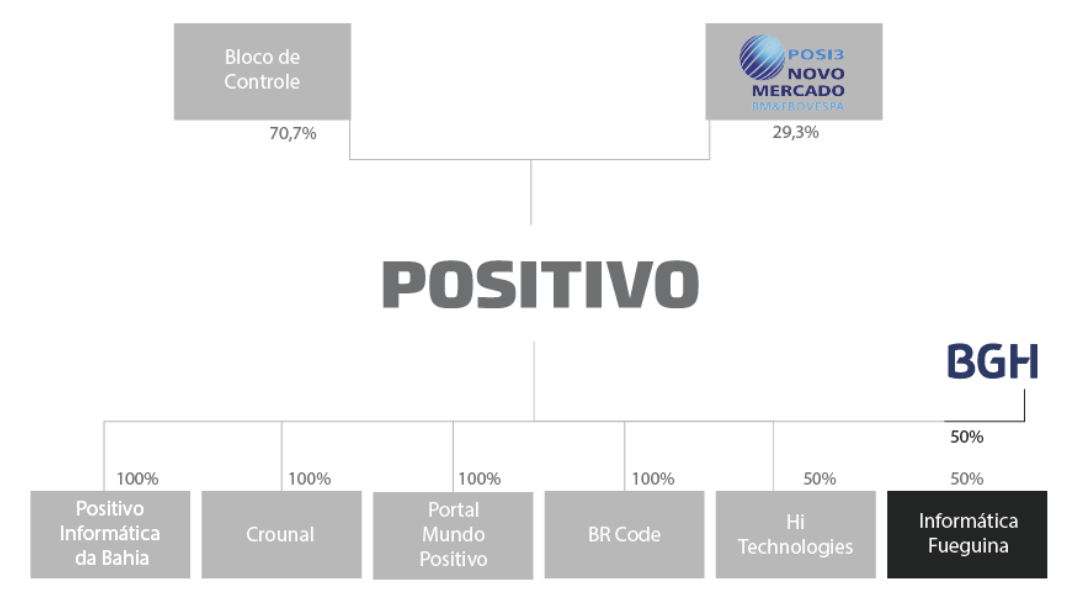
\includegraphics[width=1.0\textwidth]{Img/Corporativo}
\caption{Figura que demonstra o domínio e capital social da \nomeCompletoPositivo{}.}
\par\end{centering}
\end{figure}

Em 2016, a Positivo Tecnologia foi uma das maiores fabricantes de computadores no Brasil, respondendo por 15,3\% do número total de computadores vendidos no mercado brasileiro, de acordo com a IDC. No mesmo período, obtiveram uma participação de 19,9\% do mercado de varejo. Uma parcela substancial da produção de computadores é vendida através de grandes redes de varejo, com as quais o grupo mantém sólido relacionamento comercial, em função principalmente dos preços competitivos, do reconhecimento da marca e assistência técnica.

Adicionalmente, a companhia atua no mercado argentino por meio da marca \nomePositivoAr{}, fruto de uma joint venture com um parceiro local. Em 2015, os computadores \nomePositivoAr{} atingiram uma participação de 9,5\%, segundo a IDC.

No Brasil, a Positivo Tecnologia oferece uma linha completa de dispositivos, incluindo computadores de mesa (desktops e all-in-ones), computadores portáteis (notebooks e netbooks) e tablets, que são produzidos em Manaus (AM). Em 2012, a Companhia ingressou no mercado de telefones celulares, com a oferta de smartphones e messaging phones.

\begin{figure}[h]
\begin{centering}
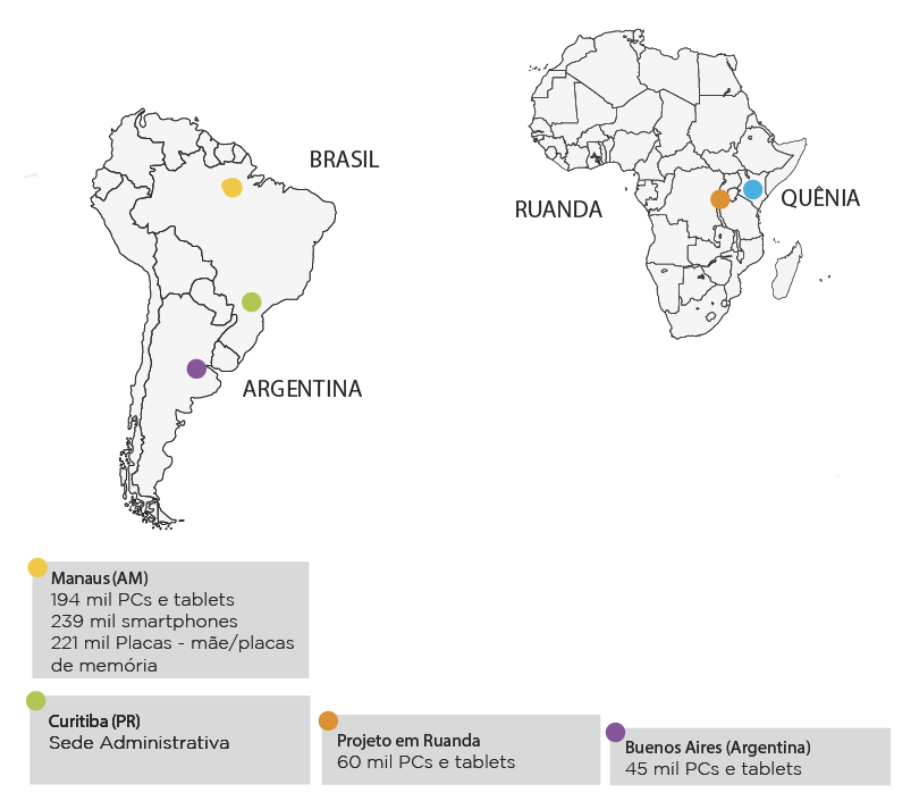
\includegraphics[width=1.0\textwidth]{Img/PositivoMundo}
\caption{Operações da \nomePositivo{} a nível mundial, bastante expressiva na América Latina e observa-se também sítios na África.}
\par\end{centering}
\end{figure}

Além disso, para atendimento e suporte aos milhões de consumidores finais, empresas e órgãos do governo, conta com uma ampla e capacitada rede de assistências técnicas cobrindo a totalidade do território nacional, e com a CRP - Central de Relacionamento Positivo, que registrou em média, 2,9 mil contatos diários em 2016. Grande parte destes contatos se refere a questões básicas sobre uso do computador, sistema operacional ou problemas com conexões, uma vez que muitos dos clientes estão adquirindo seu computador pela primeira vez.

Parcela menor da receita da Companhia provém do Segmento de Tecnologia Educacional, no qual acredita ser líder absoluto no País. A Companhia oferece soluções de infraestrutura e gestão, aplicativos e plataformas educacionais, portais de educação, além de formação de professores e acompanhamento pedagógico. Os portais têm mais de 1,2 milhões de usuários ativos, com modelo de receita recorrente mensal. 

As soluções educacionais da Positivo Tecnologia estão presentes em mais de 14 mil escolas e são exportadas para mais de 40 países. Dentre os principais produtos estão mesas educacionais, dispositivos móveis, lousas interativas, dispositivos de armazenamento e recarga, projetores, acess point, e sistema de gerenciamento de aulas. A Companhia é também distribuidor exclusivo no Brasil de empresas líderes no desenvolvimento e distribuição de software educacional, bem como distribui produtos da LEGO\texttrademark Education no território nacional.

Em 2016, a Companhia ingressou no mercado de tecnologia médica por meio da aquisição de 50\% do capital social da Hi Technologies S.A., empresa com forte foco em P\&D para a oferta de produtos inovadores em saúde.


%Adiciona introdução com numeração
% ----------------------------------------------------------
% Ficha de Avaliação Individual da Experiência Pessoal Durante Pesquisa de Campo
% ----------------------------------------------------------
%\chapter[Introdução]{Introdução}
% ---

\chapter{State of the Art}
% ---
\label{chap:literature_review}

In the following chapter, the state of the art in the lung cancer screening and incidental lung nodule care gaps and follow up literature are reviewed and discussed.

\section{Keywords and Thresholds}
\begin{center}
\begin{table}

  \begin{tabular}{c|c|c}
    \hline 
    Concept & Keywords & Articles Threshold\tabularnewline
    \hline 
    tabagism & lung nodule tabagism OR lung cancer tabagism & First 8\tabularnewline
    guidelines & lung screening guideline OR lung cancer guideline & First 8\tabularnewline
    lung cancer & lung cancer OR malignant lung nodule & First 8\tabularnewline
    imaging & dicom OR incidental lung nodule reports & First 4\tabularnewline
    nlp & natural language processing AND cancer & First 4\tabularnewline
    \hline 
  \end{tabular}
\par
\caption{\label{table:search_terms} Search terms}
\end{table}
  \vspace*{-44pt}
\end{center}

The table \ref{table:search_terms} show all the search terms utilized as a basis to extract key articles from Google Scholar, Springer  and ScienceDirect resources. For each of these articles, the most interesting related documents were also taken into account.

For each of these articles, guidelines, books and documents evaluated only the first eight of each combined search was kept as a result. All were read and the most impacting related works were also taken into consideration for this systematic literature review.

So for only the three different combined search parameters, 32 papers were selected. From these each, the  most impacting cited ones were taken into consideration, increasing the number of papers to  read to 72. From this overall number, 21 were selected to be cited as part of the literature review. % TODO

\section{Lung Cancer Studies}

Lung Cancer is the type of 30\% of all cancers. From these 30\%, 90\% of these cancers are  caused by the fact that the patient is an active or recent smoker \cite{jaklitsch2012}\cite{nccn2019}\cite{roberts2013}. This is an important literature finding because it means that patients that are effective smokers will have much greater chance of developing lung cancer than other patients.

Not only that, but other studies found out that the average quit ratio on the entire smoker worldwide population is of 7\% only but when lung  cancer screening is taken into consideration, about 25\% of the patients that start in screening program are likely to quit smoking \cite{fox2003}\cite{aalst2010}. %TODO - smoking cessation paper too

\section{Imaging Lung Nodules}

Some of the papers mention the existence of a strong correlation between patient survivability for the first 24 months and the cancer development stage. It is so common to use cancer stage (I to IV) as a proxy for survivability that there are even works whose main focus is to uncover these relations\cite{roberts2013}\cite{fox2003}.

The extensive usage of low-dose computed tomography (LDCCT) scans are also the reason for up a 20\% increase in patient survivability for the first two years of the disease development\cite{fox2003}\cite{macredmond2006}\cite{mountain2008}\cite{jaklitsch2012}. The efficiency of such early stages screening programms for LDCCT was first shown by \citeonline{henschke1999} as part of the Early Lung Cancer Action  Project (ELCAP). In this project, Chest X-ray (CXR) had an overall efficiency of 68\% and LDCCT had a 95\% for non-calcified nodules. Malignant nodules were found in 27\% of LDCCT and only 7\% for CXR. 

Other works have not only focused on the efficiency and the role of imaging but also ono the patient risk profile which is strictly related to smoking behavior.

\section{The Role of Tabagism}

Tabagism stands as the root cause for 90\% of all lung cancers. There is an increased patient risk of developing lung cancer even for patients that smoke \cite{ostroff2001}\cite{aalst2010}\cite{aalst2011}. There is definitely incidence among never smokers too but it occurs with a much lesser frequency and develops slower, mostly if the patient quits smoking before or during the radiotherapy treatment \cite{fox2003}\cite{rivera2016}

Data on tabagism is often reported for some of the patients that happen to come for Chest X-ray and Chest CT (CCT). These patients will with frequency fill up forms that amongst other informations will also extract if the patient is a smoker or not, what he or she smokes and the quantity per year. This is also true for \nomeHsl{}. 

\section{Extracting Information from Reports}

Not all patient information is stored in the form of a structured form or in a restricted text field. That means that to extract valuable information insights from the radiology reports, the anatomy patalogy reports and so on it is necessary to make extensive use of Natural Language Processing (NLP). %TODO citations

It is a known  fact that most of the medical data, altough in digital format since decades, is still in free text fields. %TODO citations
So, additional data processing is indeed necessary to provide the basis for the extraction of actionable data from the reports.

\citeonline{fleischner2017} have defined the Fleischner 2017 radiology guideline that aims to provide a patient follow-up scenario in the case of an incidental nodule finding for it. \nomeHsl{} uses Fleischner extensively for all CCT and CXR. These two procedures constitute one of the most basic imaging procedures and they do correspond to almost 20\% of all imaging done at \nomeHslShort{}. %TODO

The Fleischner guideline defines different criteria depending on the lung nodule findings in the radiology reports. These criteria are displayed at tables \ref{tab:solid_nodules} and \ref{tab:subsolid_nodules} in detail. Each of the radiology findings could potentially have a follow-up that could or not occur in time.

\begin{center}
\begin{table}
\begin{centering}
\begin{tabular}{c|>{\centering}p{0.25\textwidth}|>{\centering}p{0.25\textwidth}|>{\centering}p{0.25\textwidth}}
\hline 
\multicolumn{4}{c}{Single}\tabularnewline
\hline 
Risk & $<6mm$ & $6-8mm$ & $>8mm$\tabularnewline
\hline 
Low Risk & No routine follow-up & CT at 6-12 months, then consider CT at 18-24 months & Consider CT at 3 months, PET/CT or tissue sampling\tabularnewline
High Risk & Optional CT at 12 months & CT at 6-12 months, then consider CT at 18-24 months & Consider CT at 3 months, PET/CT or tissue sampling\tabularnewline
\hline 
\multicolumn{4}{c}{Multiple}\tabularnewline
\hline 
Low Risk & No routine follow-up & CT at 6-12 months, then consider CT at 18-24 months & CT at 6-12 months, then consider CT at 18-24 months\tabularnewline
High Risk & Optional CT at 12 months & CT at 6-12 months, then consider CT at 18-24 months & CT at 6-12 months, then consider CT at 18-24 months\tabularnewline
\hline 
\end{tabular}
\par\end{centering}
\caption{\label{tab:solid_nodules} \emph{Solid nodules} follow-up table according to \citeonline{fleischner2017}.}
\end{table}
\vspace*{-44pt}
\par\end{center}

\begin{center}
\begin{table}
\begin{centering}
\begin{tabular}{c|>{\centering}p{0.35\textwidth}|>{\centering}p{0.35\textwidth}}
\hline 
\multicolumn{3}{c}{Single}\tabularnewline
\hline 
Risk & $<6mm$ & $\geq6mm$\tabularnewline
\hline 
Ground Glass & No routine follow-up & Consider CT at 3 CT at 6-12 months to confirm persistence, then CT
every 2 years until 5 years\tabularnewline
Part Solid & No routine follow-up & Consider CT at 3 months, PET/CT or tissue sampling\tabularnewline
\hline 
\multicolumn{3}{c}{Multiple}\tabularnewline
\hline 
High Risk & CT at 3-6 months, if stable consider CT at 2 and years & CT at 3-6 months. Subsequent management based on most suspicious node(s)\tabularnewline
\hline 
\end{tabular}
\par\end{centering}
\caption{\label{tab:subsolid_nodules}\emph{Subsolid nodules} follow-up table according
to \citeonline{fleischner2017}.}
\end{table}
\vspace*{-44pt}
\par\end{center}

These follow-ups should occur as a  means of mitigating the risk that the risk of finding a malignant cancer in a late stage of clinical evolution. Missed follow-ups, as mentioned in  the chapter \ref{chap:introduction} are one of the possible medical errors. These are especially common when taking radiology reports into consideration. The reason for it is that the ordering or referring physician for the image exam forgets or does not reads the incidental lung nodule finding. 

So it would be appropriate to have any tool to help both the ordering or referring physician and the responsible physician at \nomeHsl{}. This holds true as about one third of \nomeHslShort{} workforce is constituted of external physicians, decreasing precision medicine returns values for itself. For that matter, the use of the information stored at \nomeHslShort{} has the potential of solving a potential care gap. 

\section{Differentiating Risks}

As mentioned in the previous sections, the existence of both a radiology report based risk profile and the follow-up table depending basically on the lung nodule type and  size (tables \ref{tab:solid_nodules} and \ref{tab:subsolid_nodules}). 

The patient family history of cancer and also it's smoking behavior and age should provide insight on wether the patient should be screened or not and that is the endgoal of this work.



\chapter{Data Silos, Methodology \& Results}
\label{chap:methodology}

Será utilizada a linguagem de programação Python, para a extração dos dados através de web scraping realizado em sites que possuem a geolocalização dos empreendimentos dos ativos. Estes sites contém informações de todos FIIs listados na Bolsa de Valores (B3), seus respectivos ativos imobiliários e o histórico de seus rendimentos.

Com os dados extraídos e tratados, o estudo visa criar um mapa do território brasileiro onde estarão dispostos os imóveis dos fundos e suas respectivas localizações representadas por marcadores. Os marcadores serão distinguidos por cores, onde cada cor representará o FII a qual ele pertence e o seu tamanho demonstrará a renda/valorização do fundo. A partir desta visualização o estudo tende a criar um ambiente de maior visualização e análise.

\section{Extração por \emph{Webscrapping}}
\label{sec:extraction_by_webscrapping}
\begin{table}
\begin{centering}
\csvautobooktabular {\tablePath/ImovelPorEstado.csv}
\caption{\label{tab:papers_per_state} Número de ativos de imóveis por estado para os 118 fundos imobiliários analisados.}
\end{centering}
\end{table}

Foi extraído os dados dos fundos imobiliários do site \emph{fundsexplorer}. Excluímos todos os fundos com volume médio igual a zero e com missing values, pois estes podem ter sido incorporado por outros, duplicando assim os ativos.

Obteve-se então uma base de 118 fundos imobiliários no Brasil, destes, 74 tem 390 ativos divididos em 19 estados e 123 cidades.  O resultado final pode ser observado na tabela~\ref{tab:papers_per_state}, ordenada pela quantidade de papeis em cada estado. Notadamente, São Paulo possui grande destaque com 56\% dos ativos, seguido pelo Rio de Janeiro com 17\%. No total, a região sudeste corresponde a 81\% dos ativos.

Após extrair-se as informçães obteve-se o \emph{dataset} de ativos na seguinte estrutura~\ref{tab:example_papers}. Observa-se que esta estrutura contém diversos endereços e em alguns casos múltiplos endereços na mesma linha. Por este motivo, foi necessário tratar-se os dados obtidos, conforme demonstrado na figura~\ref{fig:geoencoding_and_problems}.

\begin{table}
\begin{centering}
%\csvautobooktabular[separator=pipe]{\tablePath/ExemplosAtivos.csv}
\begin{tabular}{l>{\raggedright}p{0.12\textwidth}>{\raggedright}p{0.2\textwidth}>{\raggedright}p{0.15\textwidth}l>{\raggedright}p{0.1\textwidth}>{\raggedright}p{0.12\textwidth}}
\hline 
Fundo & Título & Endereço & Bairro & UF & Cidade & Área(\texttwosuperior{})\tabularnewline
\hline 
ABCP11 & Grand Plaza Shopping & Av. Industrial, 600 & Tamanduateí 3 & SP & Santo André & 69.628\tabularnewline
AEFI11 & Campinas & Avenida John Boyd Dunlop, s/n & Jardim Ipaussurama & SP & Campinas & 96.435,16 \tabularnewline
AEFI11 & Cuiabá & Avenida Fernando Corrêa da Costa, s/nº & Nossa Senhora Aparecida & MT & Cuiabá & 25.000 \tabularnewline
AGCX11 & Ag 14 Bis & Av. Marechal Câmara, 160 & Centro & RJ & Rio de Janeiro & 1.900,31 \tabularnewline
AGCX11 & Ag Av Chile & Av. República do Chile, 230 & Centro & RJ & Rio de Janeiro & 1.139,67 \tabularnewline
AGCX11 & Ag Av. Pres. Wilson & Av. Rio Branco, 311-B & Centro & RJ & Rio de Janeiro & 713,62 \tabularnewline
AGCX11 & Ag Bandeira & R. Mariz e Barros, 79 (Loja) & Praça da Bandeira & RJ & Rio de Janeiro & 1.339 \tabularnewline
AGCX11 & Ag Barra Funda & Av. Rio Branco, 1675 (Loja) & Campos Eliseos & SP & São Paulo & 1.293,02 \tabularnewline
AGCX11 & Ag Benedito Coutinho & R. Antônio Bernardo Coutinho, 163 & Centro & SP & Osasco & 1.206,10 \tabularnewline
AGCX11 & Ag Campo Limpo & Est. do Campo Limpo, 5520 & Vila Pirajussara & SP & São Paulo & 604 \tabularnewline
AGCX11 & Ag Capão Redondo & Estrada de Itapecerica, 3429 & Vila Maracana & SP & São Paulo & 1.448,48 \tabularnewline
AGCX11 & Ag Estrada Rio do A & Est. Rio do A, 1131 &  & RJ & Campo Grande & 571,41 \tabularnewline
AGCX11 & Ag Guaianases & R. Salvador Gianetti, 436 & Guaianases & SP & São Paulo & 2.475,10 \tabularnewline
AGCX11 & Ag Guarapiranga & Av. de Pinedo, 228 & Capela do Socorro & SP & São Paulo & 1.312,18 \tabularnewline
AGCX11 & Ag Hebraica & Av. Brigadeiro Faria Lima, 1644 & Jardim Paulistano & SP & São Paulo & 323,31 \tabularnewline
AGCX11 & Ag Inconfidencia & R. Curitiba, 888 & Centro & MG & Belo Horizonte & 2.373,17 \tabularnewline
\dots{} & \dots{} & \dots{} & \dots{} & \dots{} & \dots{} & \dots{}\tabularnewline
\hline 
\end{tabular}
\caption{\label{tab:example_papers}Exemplos de Ativos extraídos pela utilização de técnicas de \emph{webscrapping}}
\end{centering}
\end{table}

Geocodificamos o endereço dos ativos através do GoogleEarth e obtivos um arquivo .kml. Em sequência, os dados foram importados no software QGis e ao plotar-se os diversos ativos sobre o mapa dos estados da federação obteve-se a figura \ref{fig:papers_vs_dividends}.

\begin{center}
\begin{figure}
\begin{centering}
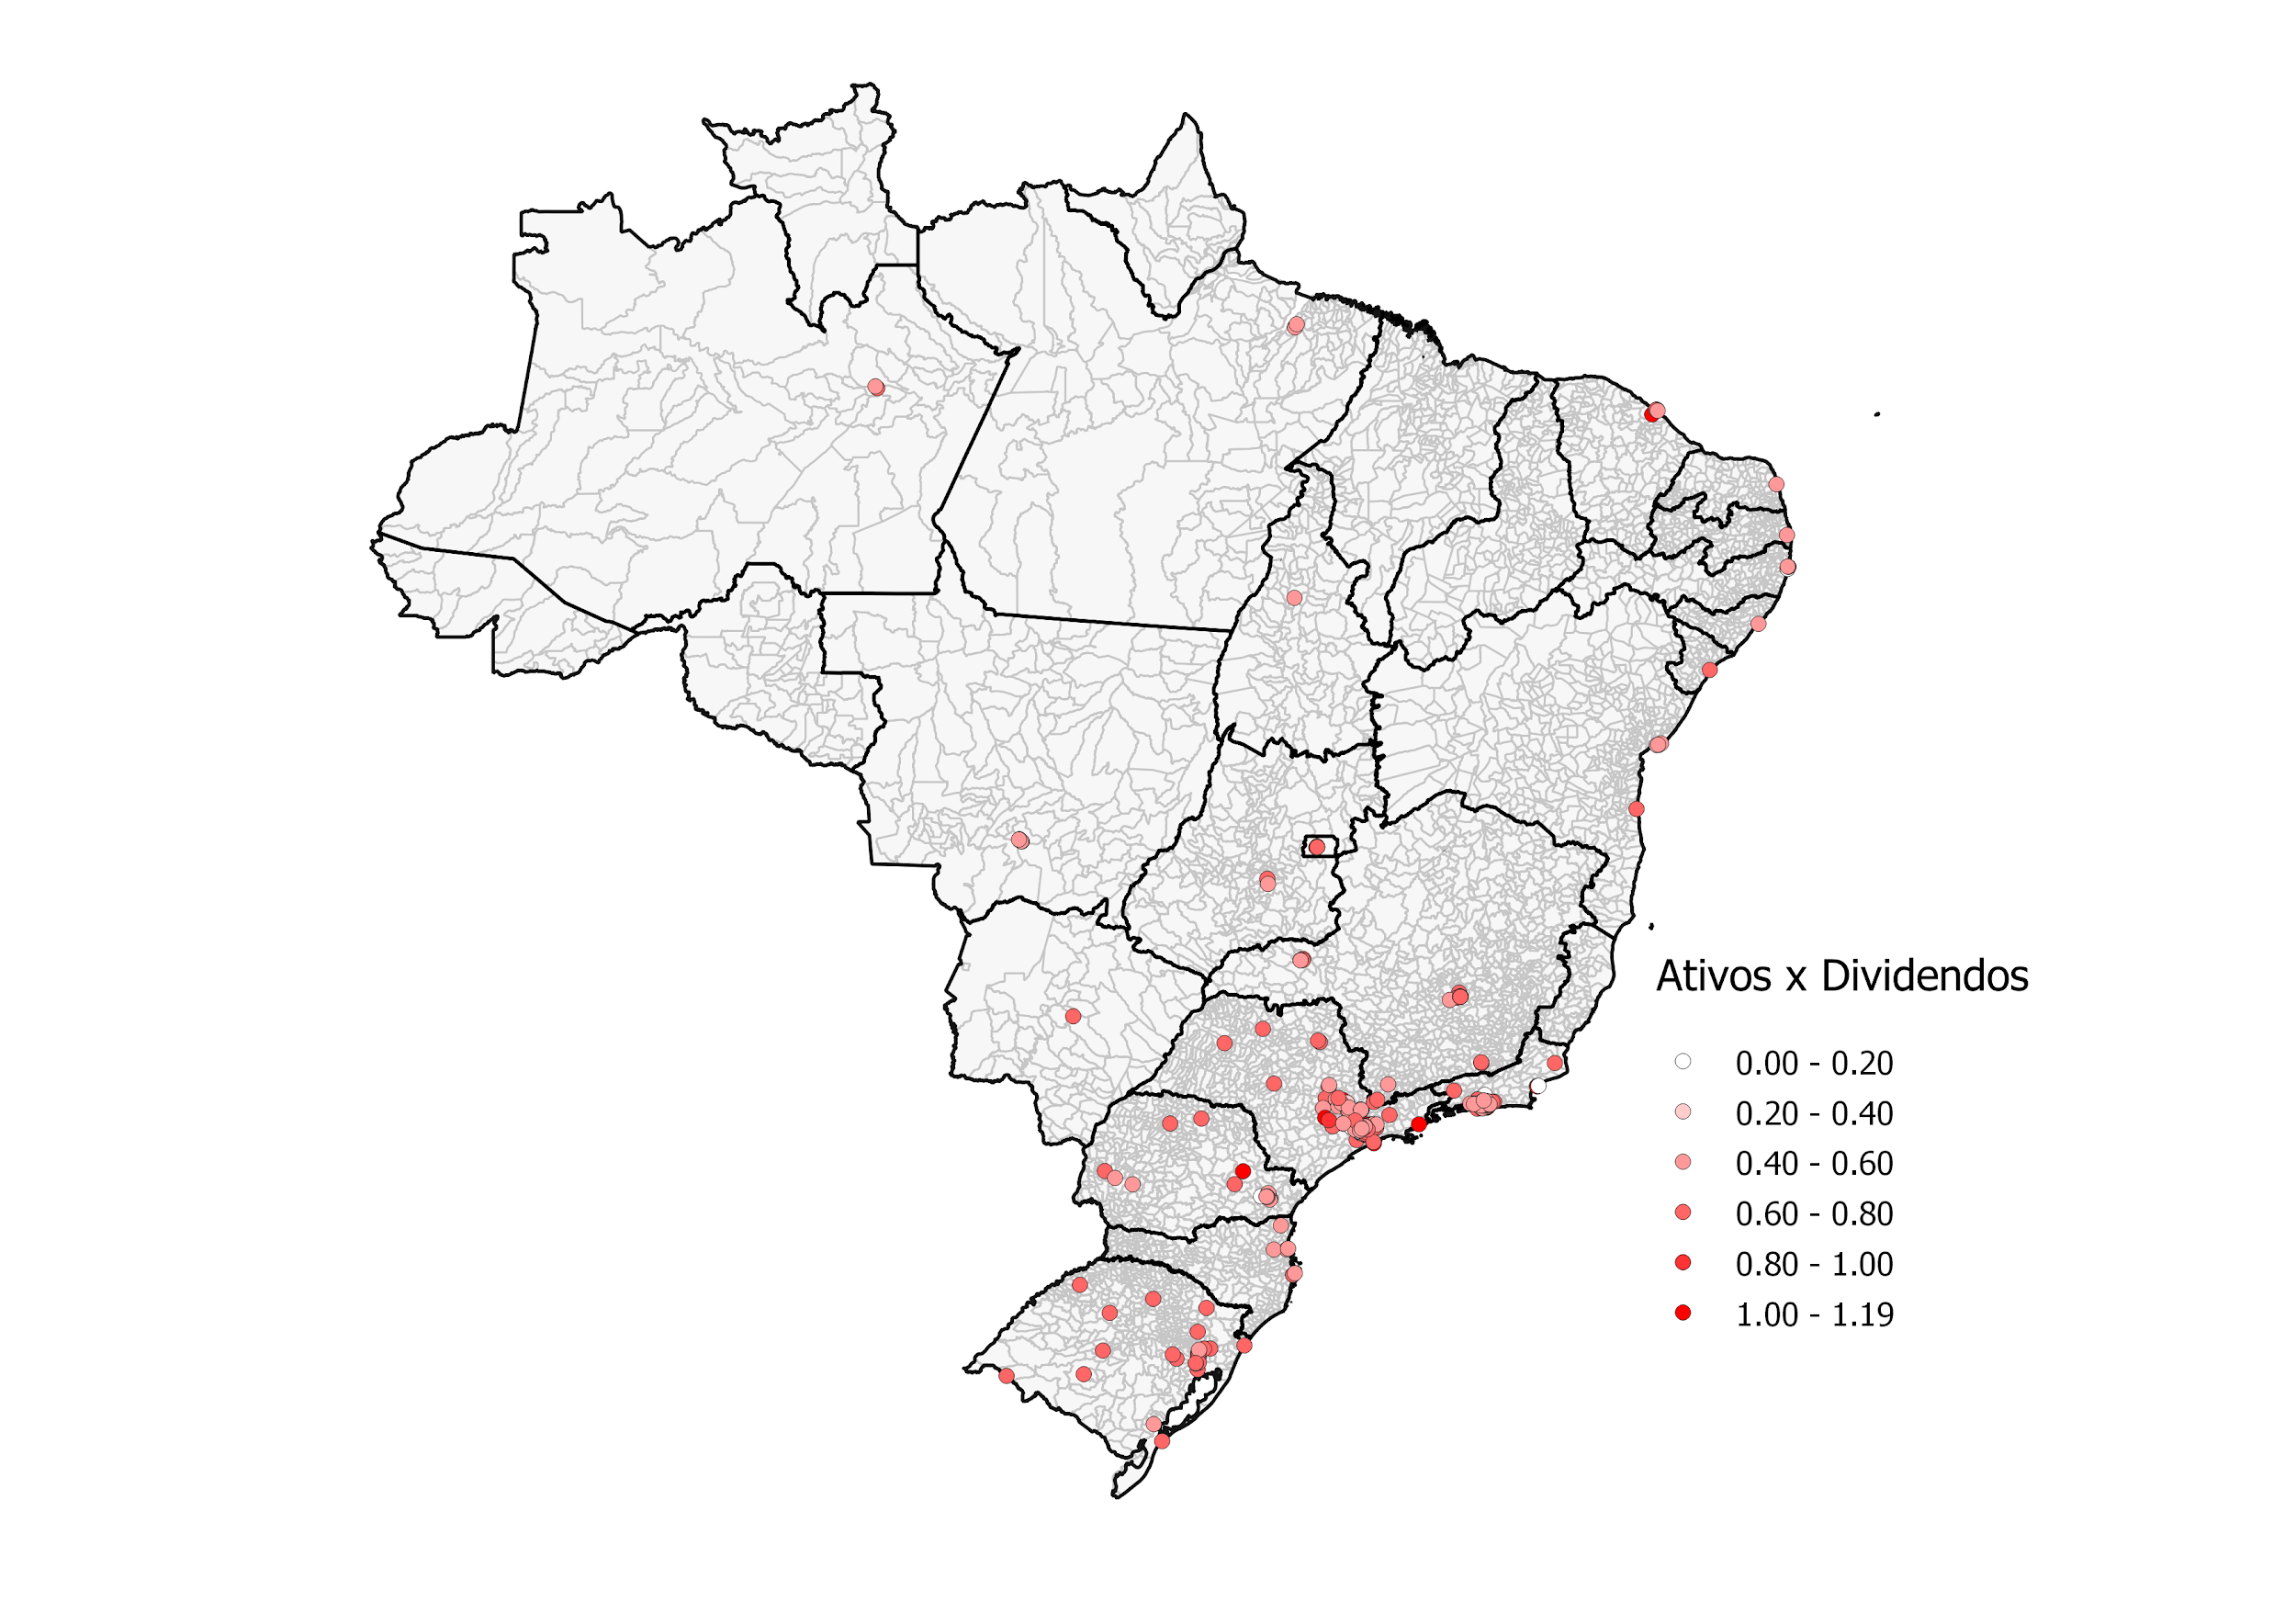
\includegraphics[width=1.0\textwidth]{AtivosxDividendosPorEstados}
\end{centering}
\caption{\label{fig:papers_vs_dividends}Os 118 ativos imobiliários em relação aos dividendos obtidos para o ano 2018/2019.}
\end{figure}
\vspace*{-44pt}
\end{center}

\begin{center}
\begin{figure}
\begin{centering}
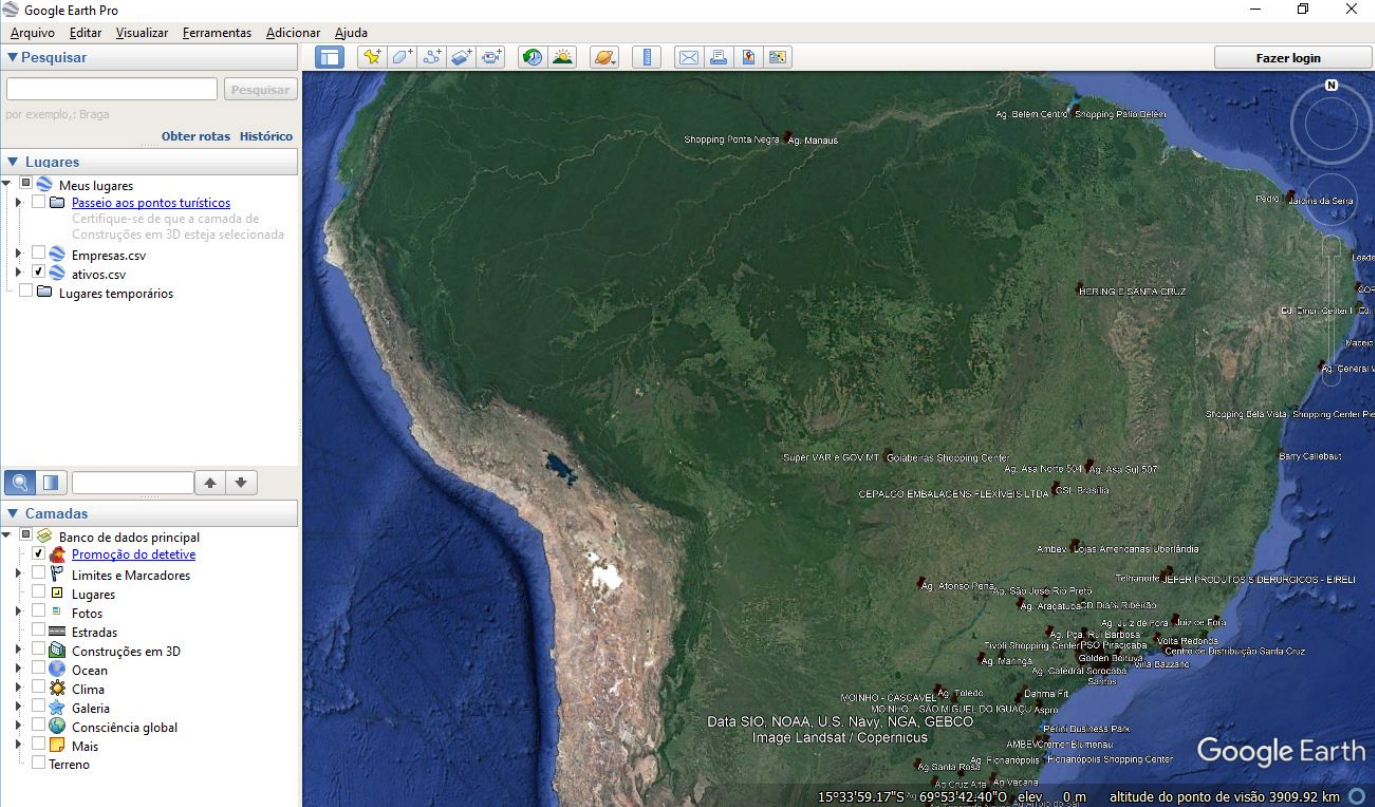
\includegraphics[width=0.85\textwidth]{GoogleEarth_Geoencoding}
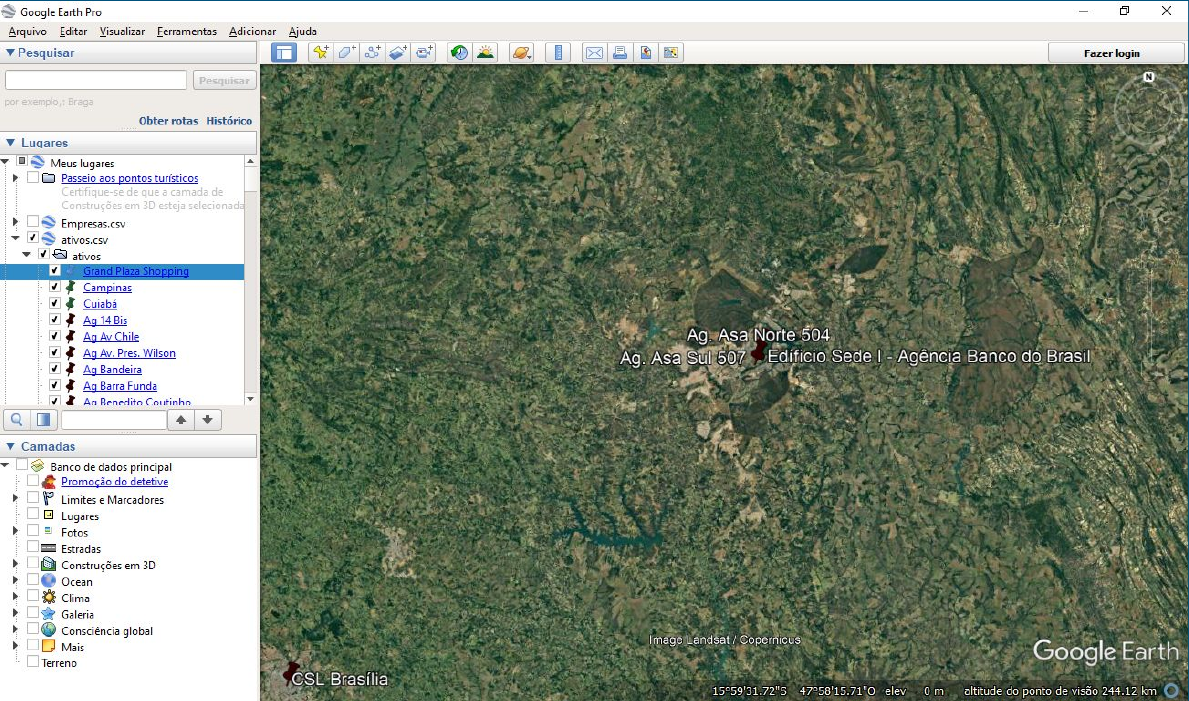
\includegraphics[width=0.85\textwidth]{GoogleEarth_GeoencodingProblems}
\end{centering}
\caption{\label{fig:geoencoding_and_problems}Processo de geocodificação no Google Earth (acima) e problemas encontrados no processamento dos endereços (abaixo).}
\end{figure}
\vspace*{-44pt}
\end{center}

O processo de geocodificação também teve seus desafios, uma vez que diversos endereços, sobretudo os da região centro-oeste, em que o Google Earth teve dificuldades de associar o endereço a uma região censitária. Um exemplo de problema de geocodificação pode ser visto na figura~\ref{fig:geoencoding_and_problems}. Logo acima, na mesma figura, encontra-se demonstrado o processo de geocodificação no Google Earth. 

Conforme mencionado, cerca de 20\% de todos os endereços apresentaram problemas. Sendo assim, foi necessário informar-se manualmente no Google Earth o endereço alvo correto.

Pode-se verificar que a maioria dos fundos se encontram-se no Sudeste e no Sul, dos fundos do sudeste, em sua maioria no estado de São Paulo, a maior concentração é no centro. No Rio Grande do Sul, os ativos estão bem espalhados, enquanto nas demais regiões do país, eles se encontram em cidades perto de cidades litorâneas. 

\begin{center}
\begin{figure}
\begin{centering}
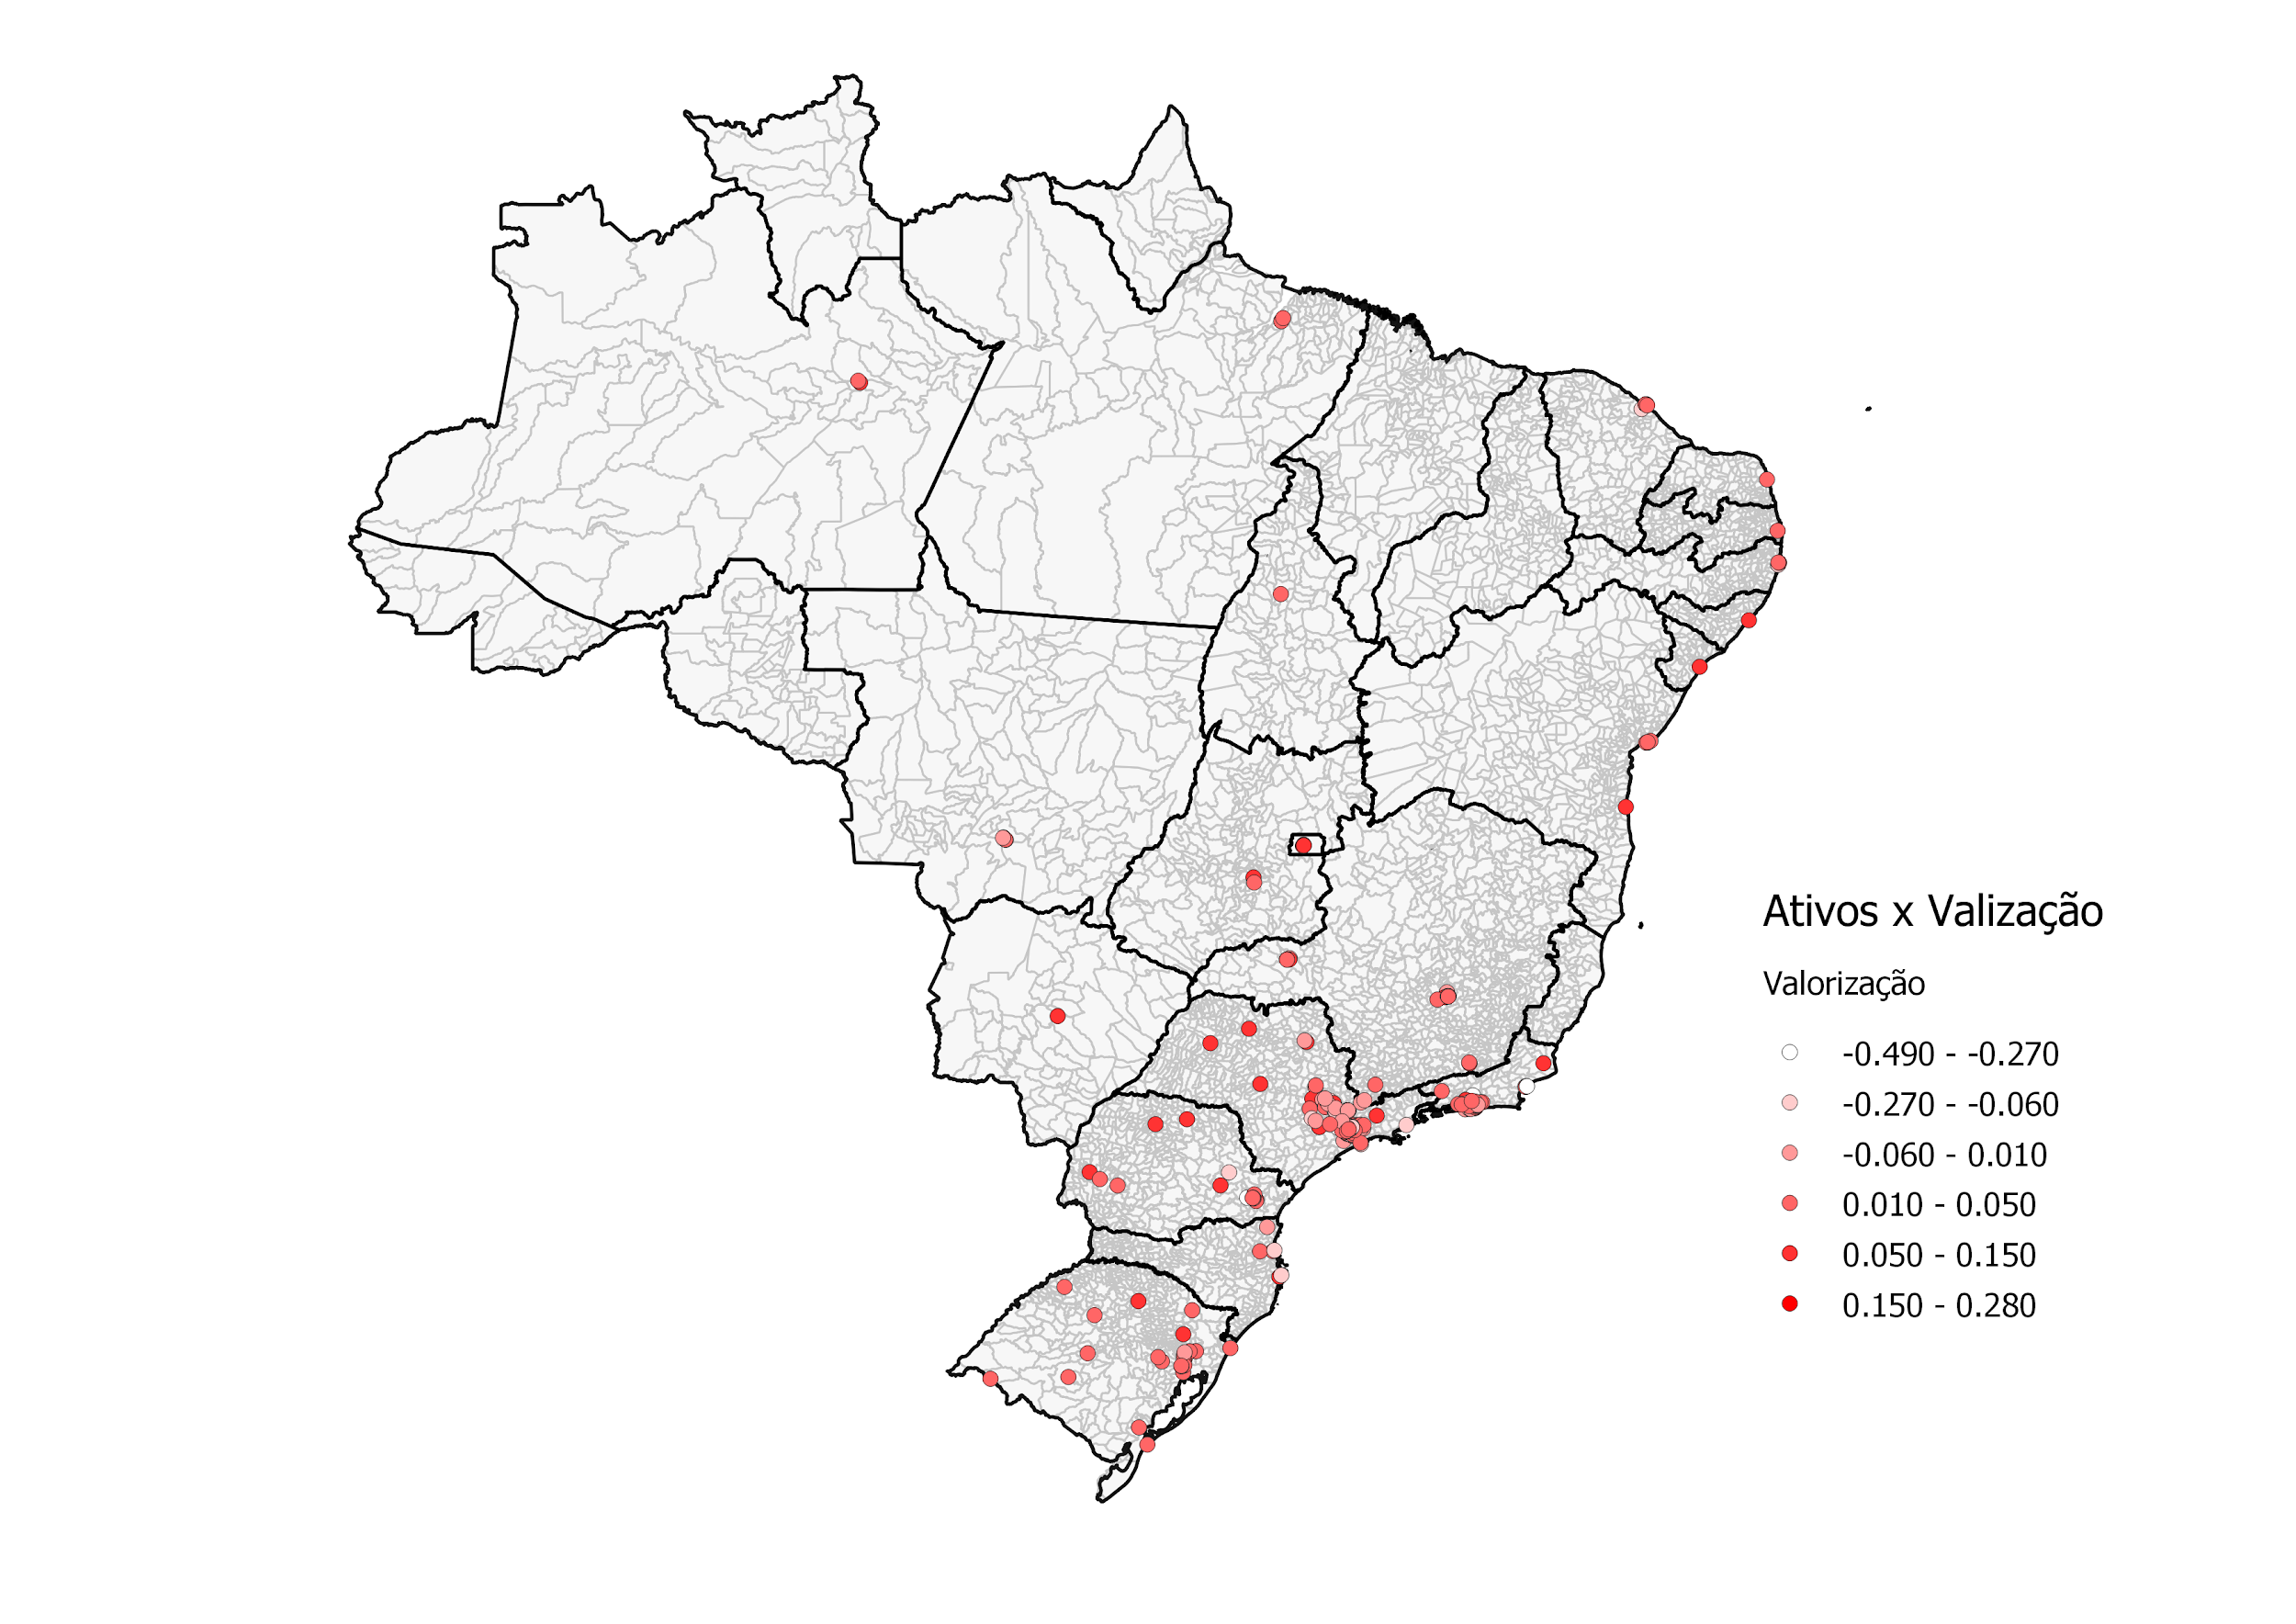
\includegraphics[width=1.0\textwidth]{AtivosxValizacaoPorEstados}
\end{centering}
\caption{\label{fig:papers_vs_valization}Os 118 ativos imobiliários em relação a valização obtida para o ano 2018/2019.}
\end{figure}
\vspace*{-44pt}
\end{center}

Esta informação casa bem com o esperado, uma vez que a concentração de pessoas e portanto de imóveis e muito maior nas cidades próximo ao litoral do que no interior do país. Nota-se também, que os fundos com maior rentabilidade são os do Sudeste, mais especificamente de São Paulo. %TODO - cite

No mapa da figura \ref{fig:papers_vs_valization}, é possível notar que existe grande correlação entre os dividendos pago pelo FII e sua valorização nos últimos 12 meses. E novamente os ativos localizado em SP, RJ e RS apresentaram maior valorização. Percebe-se assim que há uma possível relação espacial entre a localização geográfica de um ativo imobiliário e sua valorização no ano referente.

\section{Variáveis Iniciais}
\label{sec:initial_variables}
\begin{table}[h]

\begin{centering}
  \csvautobooktabular[separator=pipe]{\tablePath/VariaveisIniciais.csv}
\caption{\label{tab:initial_variables} Variáveis relacionadas aos Fundos de Investimentos Imobiliários de interesse para a análise do trabalho.}
\end{centering}
\end{table}

Na tabela \ref{tab:initial_variables}, demonstram-se as variáveis de interesse para análise, incluindo a variável localização do ativo, usada para o georeferenciamento do mesmo.

\section{Análise Multivariada}
\label{sec:multivariate_analysis}

\begin{center}
\begin{figure}
\begin{centering}
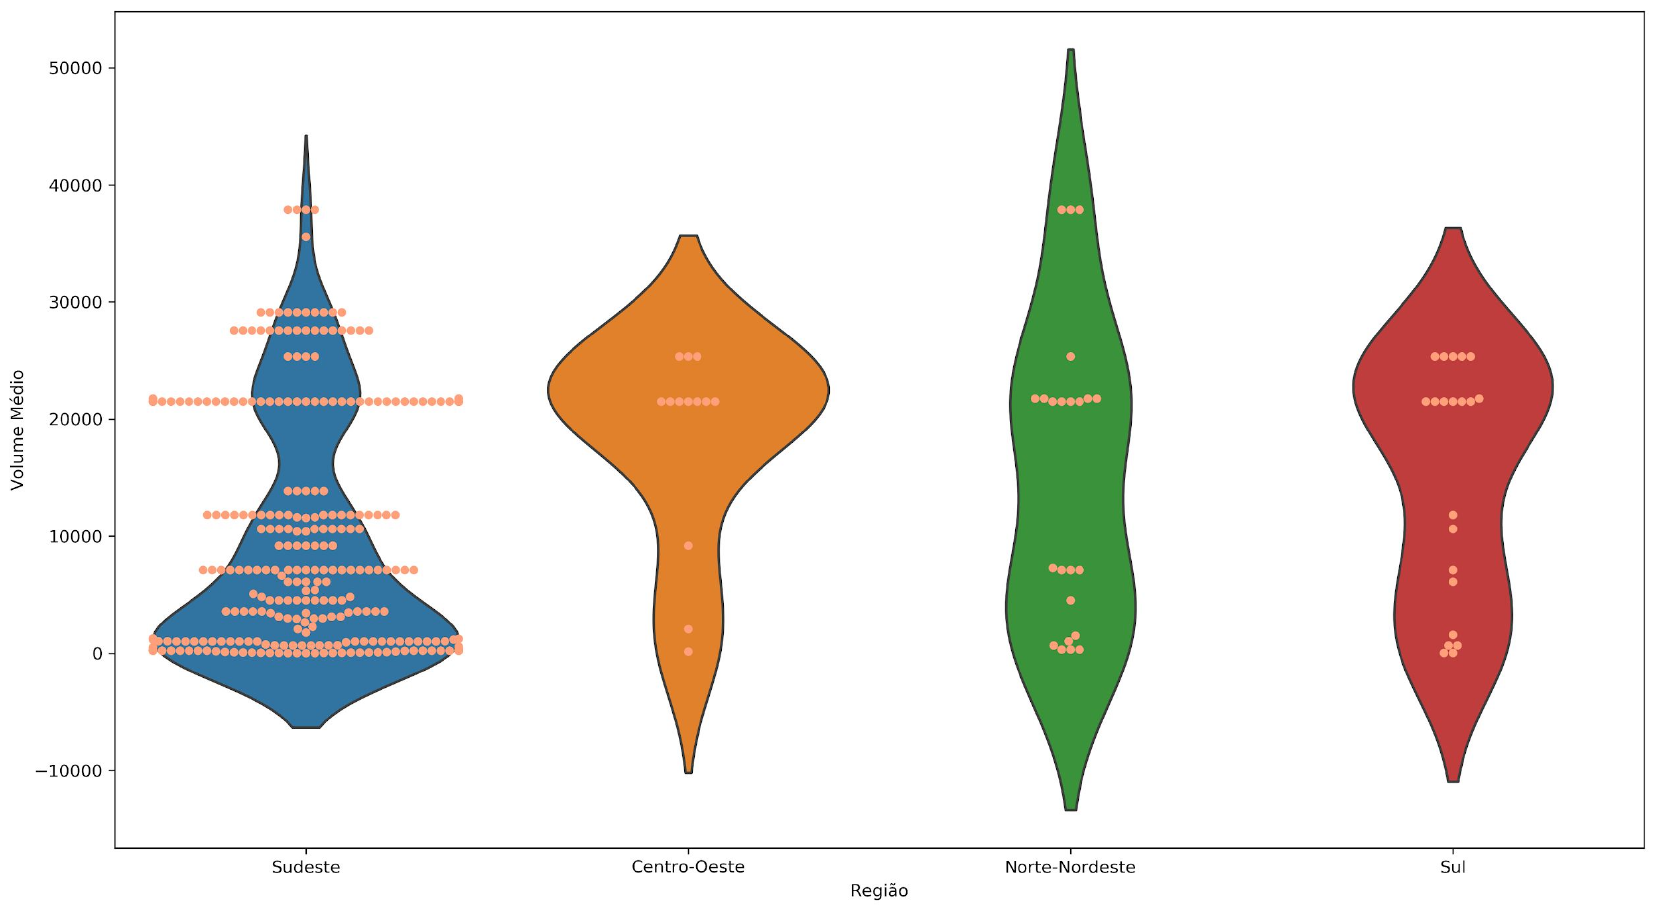
\includegraphics[width=1.0\textwidth]{RegionsPerVolume}
\end{centering}
\caption{\label{fig:regions_per_volume}Variável \emph{volume médio} por região. Observa-se no \emph{swarmplot} uma predominância de ativos com presença no Sudeste conforme esperado e visto na seção~\ref{sec:extraction_by_webscrapping}.}
\end{figure}
\vspace*{-44pt}
\end{center}

Realizamos uma análise multivariada utilizando as seguintes bibliotecas do python:

\begin{itemize}
  \item geocoder
  \item geopandas
  \item pandas
  \item pysal
  \item libpysal
  \item mapclassify
  \item seaborn
  \item matplotlib
\end{itemize}

\begin{center}
\begin{figure}
\begin{centering}
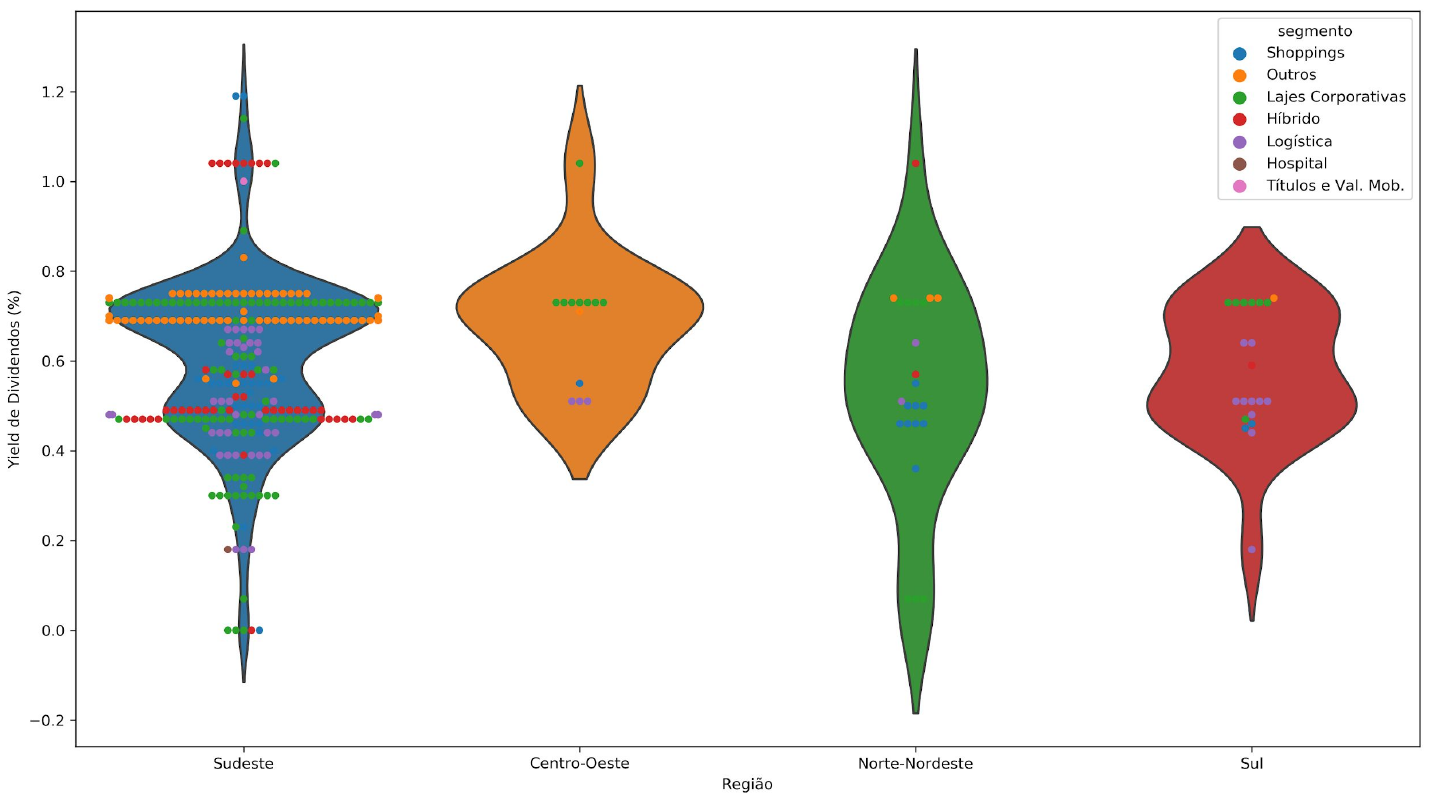
\includegraphics[width=1.0\textwidth]{RegionsPerYield}
\end{centering}
\caption{\label{fig:regions_yield}Variável \emph{yield} por região.  Os segmentos \emph{híbrido} e \emph{outros} apresentaram performance acima dos demais para a região Sudeste. Nesta mesma região \emph{lajes corporativas} possuem um retorno menor neste parâmetro.}
\end{figure}
\vspace*{-44pt}
\end{center}

Para a análise em si, inicialmente dividiu-se o Brasil nas regiões Sul, Sudeste, Centro-oeste e Norte-nordeste. Para fins de análise, tentou-se avaliar as variáveis referenciadas na seção~\ref{sec:initial_variables}. Isto é, \emph{volume médio}, $p/vp$, \emph{valorização} e \emph{yield de dividendos}.

A figura~\ref{fig:regions_per_volume} mostra o volume médio de operações mensais em relação aos ativos. Nota-se uma certa concentração de fundos sem volume, sobretudo na região \emph{Sudeste}. Isto pode ser devido tanto aos \emph{FIIs} ainda serem recentes em relação a outros investimentos mais conhecidos no mercado ou mesmo pelo fato do brasileiro não ter uma característica de investimento em papéis de maneira geral. Somente recentemente que a BOVESPA, bolsa de ações no país, passou a marca de 1 milhão de pessoas físicas cadastradas.

\begin{center}
\begin{figure}
\begin{centering}
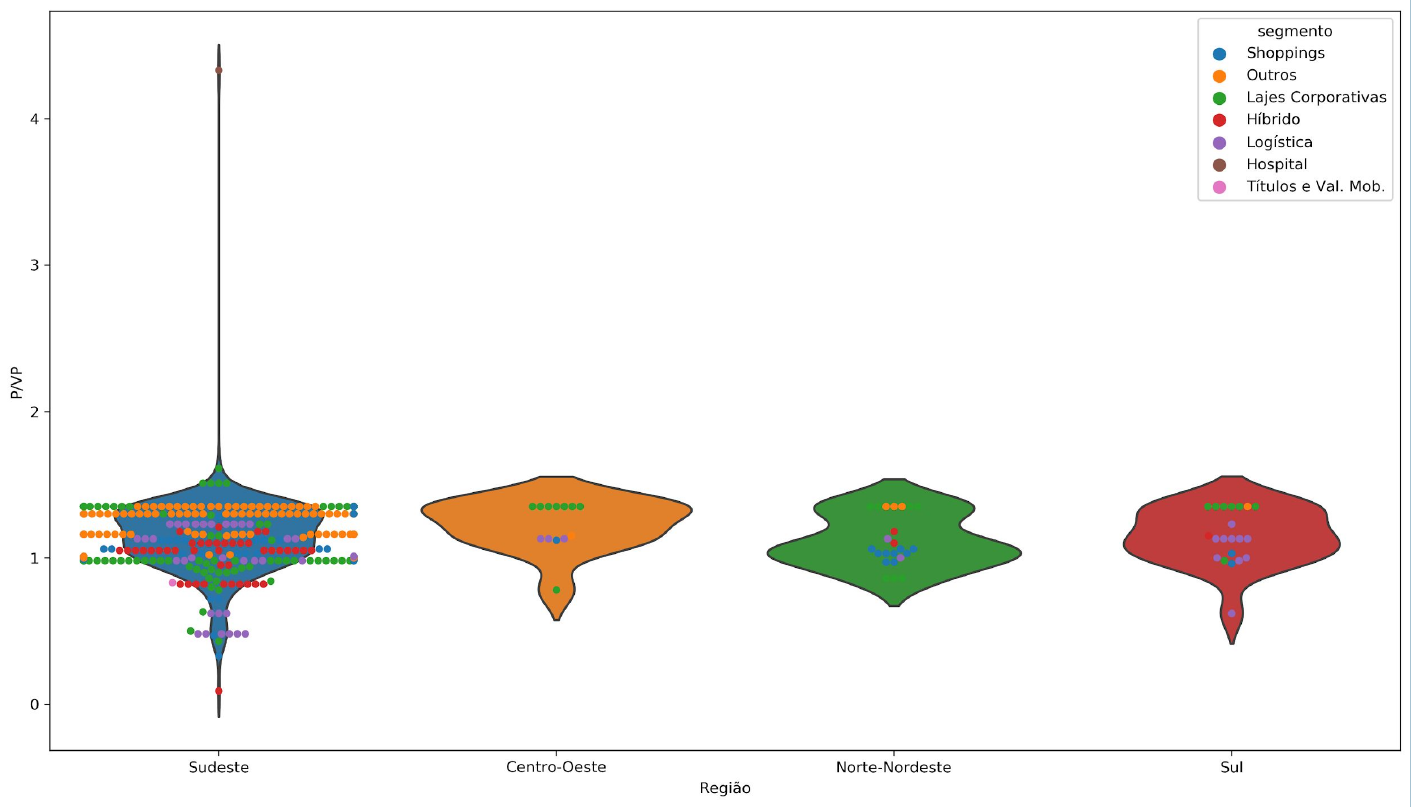
\includegraphics[width=1.0\textwidth]{RegionsPerPvp}
\end{centering}
\caption{\label{fig:regions_pvp}Variável $p/vp$ por região. Norte-nordeste é bem atrativo neste quesito.}
\end{figure}
\vspace*{-44pt}
\end{center}

Na figura~\ref{fig:regions_yield}, tem-se por cor a categoria dos fundos aos quais os ativos são pertencentes. Nota-se que na região Sudeste, mais significativa em volume de ativos, os segmentos \emph{híbrido} e \emph{outros} apresentam dividendos acima dos demais. Já \emph{lajes corporativas}, \emph{shoppings}, \emph{logística} e \emph{títulos} apresentam valores mais baixos na média. 

Com relação ao parâmetro \emph{valorização}, na figura~\ref{fig:regions_evaluation}, os segmentos que melhor desempenham são \emph{lajes corporativas} e \emph{outros}. Para a região centro-oeste, a primeira também apresenta valorização significativa.

\begin{center}
\begin{figure}
\begin{centering}
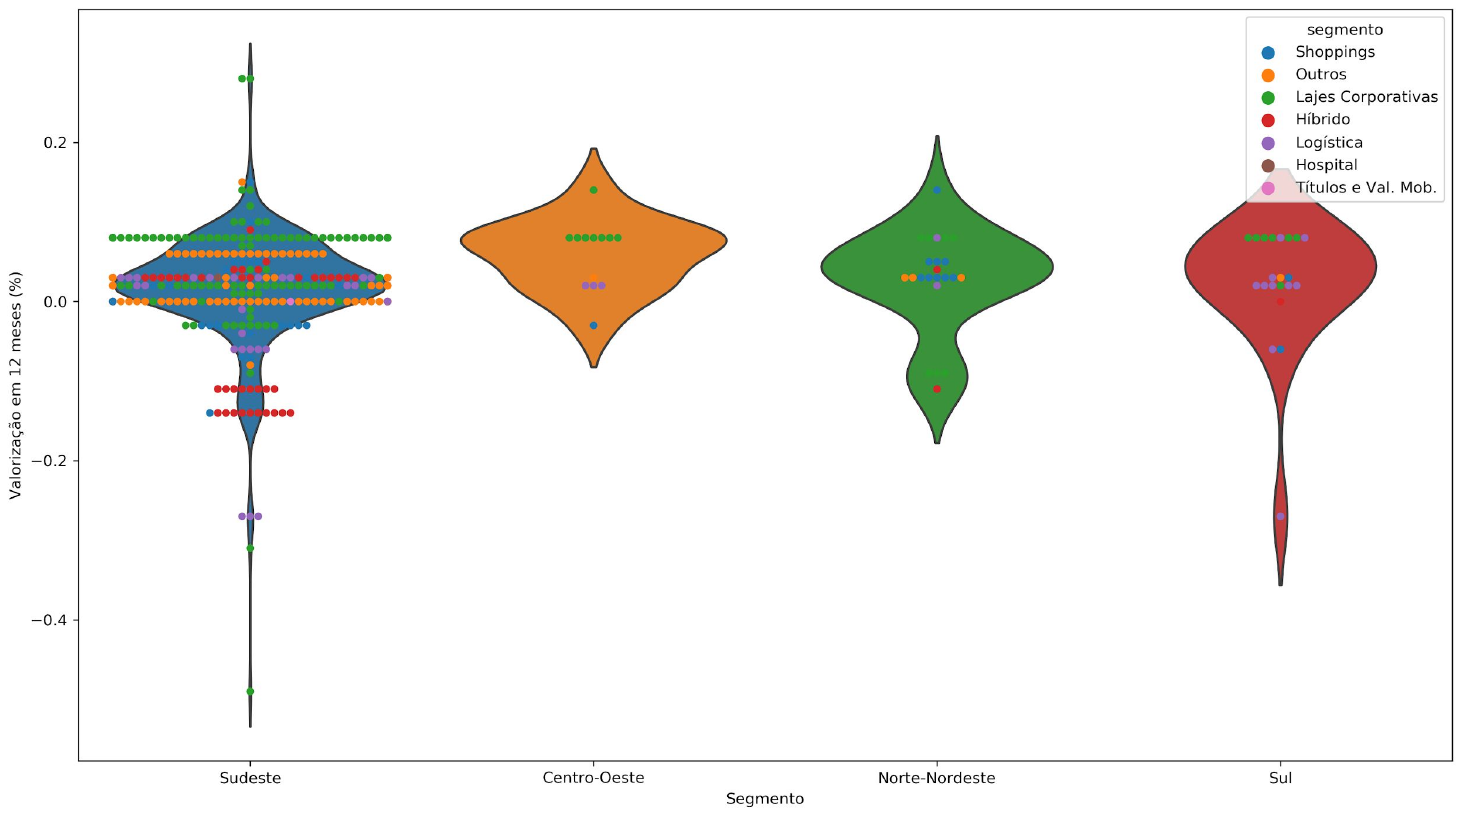
\includegraphics[width=1.0\textwidth]{SegmentPerEvaluation}
\end{centering}
\caption{\label{fig:regions_evaluation}Variável \emph{valorização} por região (12 meses). Observa-se no \emph{swarmplot} uma predominância de ativos com presença na região Sudeste.}
\end{figure}
\vspace*{-44pt}
\end{center}

Por fim, nota-se na figura~\ref{fig:regions_pvp}, que é uma variável tipicamente presente em análises fundamentalistas, onde valores acima de 1 significam valorização acima do esperado (preço alto) e valores abaixo de 1, preço baixo. Pela análise desta variável o setor de \emph{lajes corporativas}, \emph{híbrido} e \emph{logística} despontam como mais interessantes para compra na região sudeste. nas demais regiões observa-se forte valorização do preço das \emph{lajes corporativas}.

\section{Análise Espacial}
\label{sec:spatial_analysis_br}

A análise espacial de pesos é feita a partir da resolução da matriz de pesos da vizinhança de uma variável qualquer num grid regular espaçado em um quadrado \emph{n por n}. O grid $W$ é dado pela razão dos pesos dos seus vizinhos, isto é:

\[
W_{nxn}=\left[\begin{array}{cccc}
w_{11} & w_{12} & ... & w_{1n}\\
w_{21} & w_{22} & ... & w_{2n}\\
... & ... & ... &...\\
w_{n1} & w_{n2} & ... & w_{nn}
\end{array}\right]
\]

Para a matriz de pesos \emph{Queen}, de grau 1, cada peso é calculado a partir da vizinhança imediata cheia, isto é os 8 elementos adjacentes. Já o método de \emph{Rock}, prevê somente aquelas adjacentes ortogonalmente, mas não aquelas em que a adjacência seja diagonal ao elemento, isto é, em formato de cruz.

\begin{center}
\begin{figure}
\begin{centering}
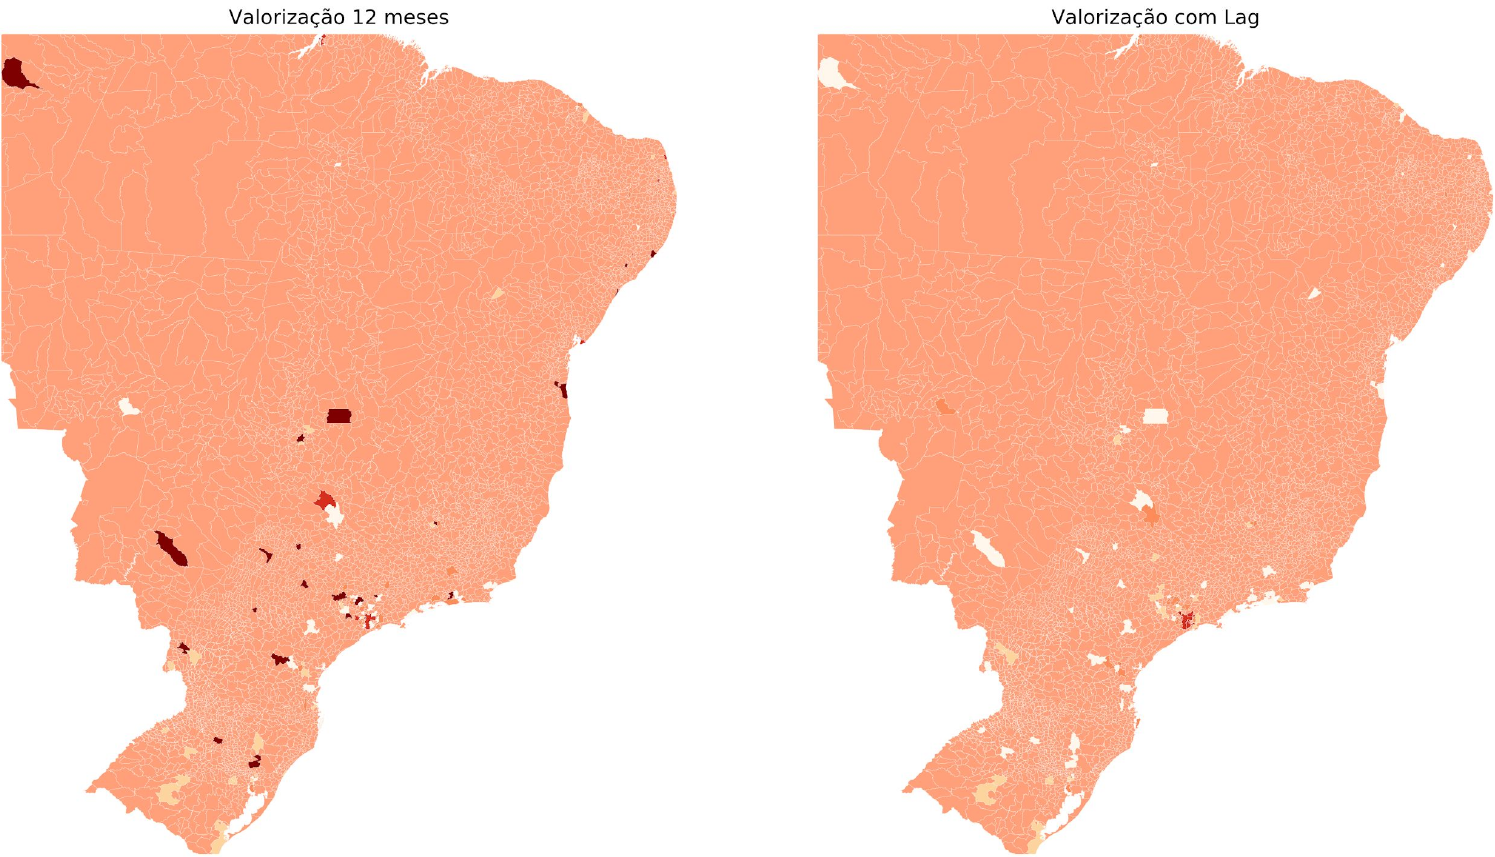
\includegraphics[width=1.0\textwidth]{EvaluationPerCensitaryRegions}
\end{centering}
\caption{\label{fig:brazil_evaluation}Valorização com relação as regiões censitárias. Do lado esquerdo a valorização absoluta e do lado direito a valorização levando em consideração a vizinhança por Queen com $n=1$ de lag.}
\end{figure}
\vspace*{-44pt}
\end{center}

Os pesos são calculados amostrando-se pelos chamados \emph{pesos padronizados por linha}, segundo a fórmula:

\[
w_{ij(s)}=w_{ij}/\sum_{j}w_{ij}
\]

Um outro fator importante já mencionado é a contiguidade que apresenta formas diferentes para o método de \emph{Queen} e \emph{Rock}. Ambos métodos são extremamente sensíveis ao fator de continuidade dos dados e por isso caso não haja um casamento adequado aos dados, é possível que seja necessário tratá-los.

\begin{center}
\begin{figure}
\begin{centering}
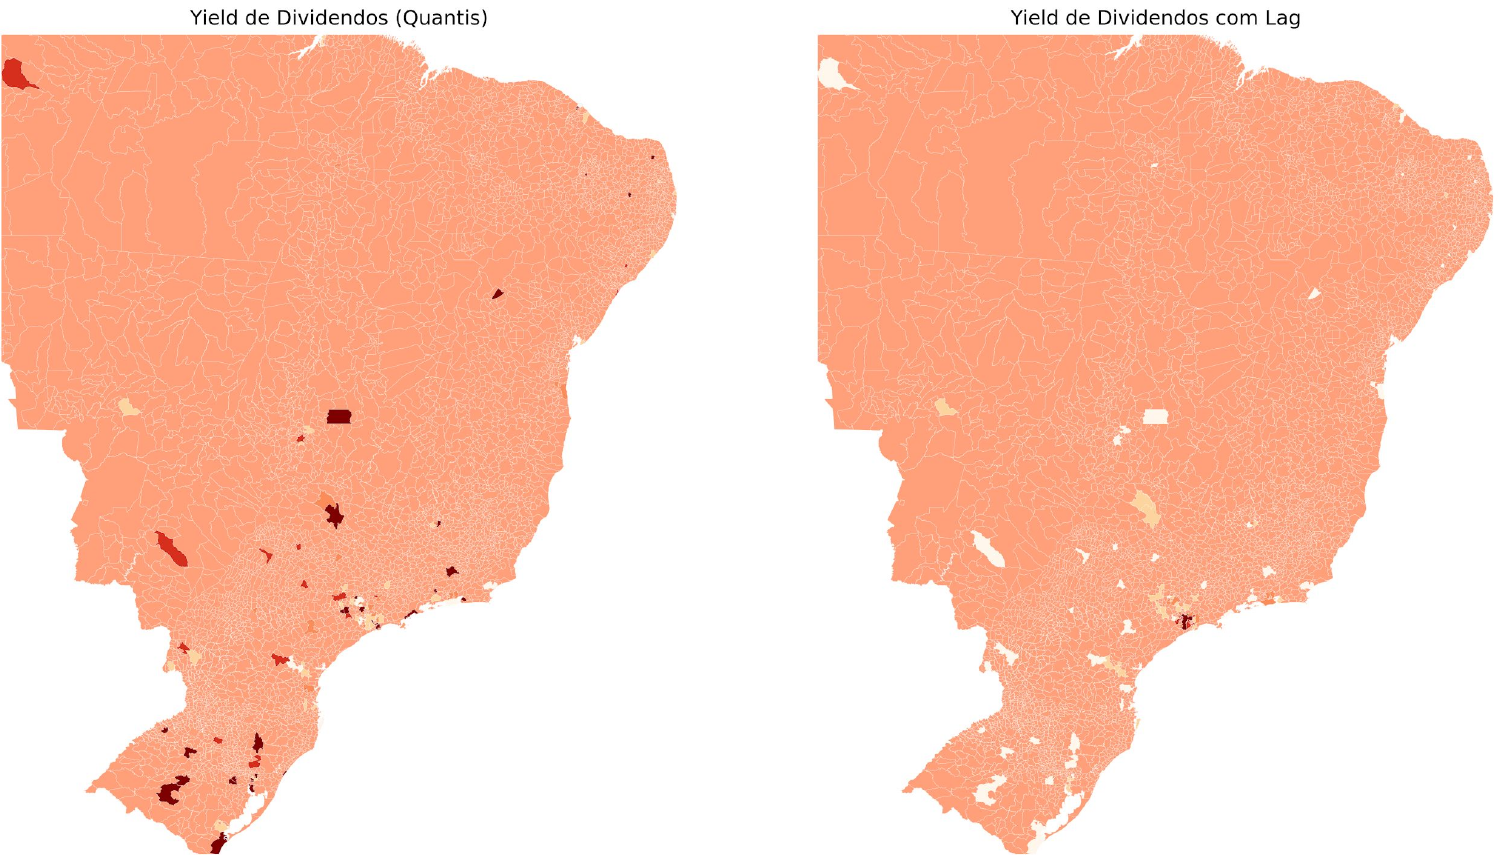
\includegraphics[width=1.0\textwidth]{YieldPerCensitaryRegionWithlag}
\end{centering}
\caption{\label{fig:brazil_yields}\emph{Yield} com relação as regiões censitárias. Do lado esquerdo a valorização absoluta e do lado direito a valorização levando em consideração a vizinhança por Queen com $n=1$ de lag.}
\end{figure}
\vspace*{-44pt}
\end{center}

As figuras~\ref{fig:brazil_evaluation} e~\ref{fig:brazil_yields} demonstram a \emph{valorização} e o \emph{yield} de cada ativo por região censitária. Em ambos os casos somente a região de São Paulo capital ainda permance com um valor significativo levando-se em consideração a vizinhança. 

Conforme mencionado anteriormente, a análise de pesos por Queen é muito sensível a densidade de dados da vizinhança. Sendo assim, decidiu-se reduzir o escopo dos ativos àqueles da região da capital paulista somente.

\section{Análise Espacial de São Paulo}
\label{sec:spatial_analysis_sao_paulo}

\begin{center}
\begin{figure}
\begin{centering}
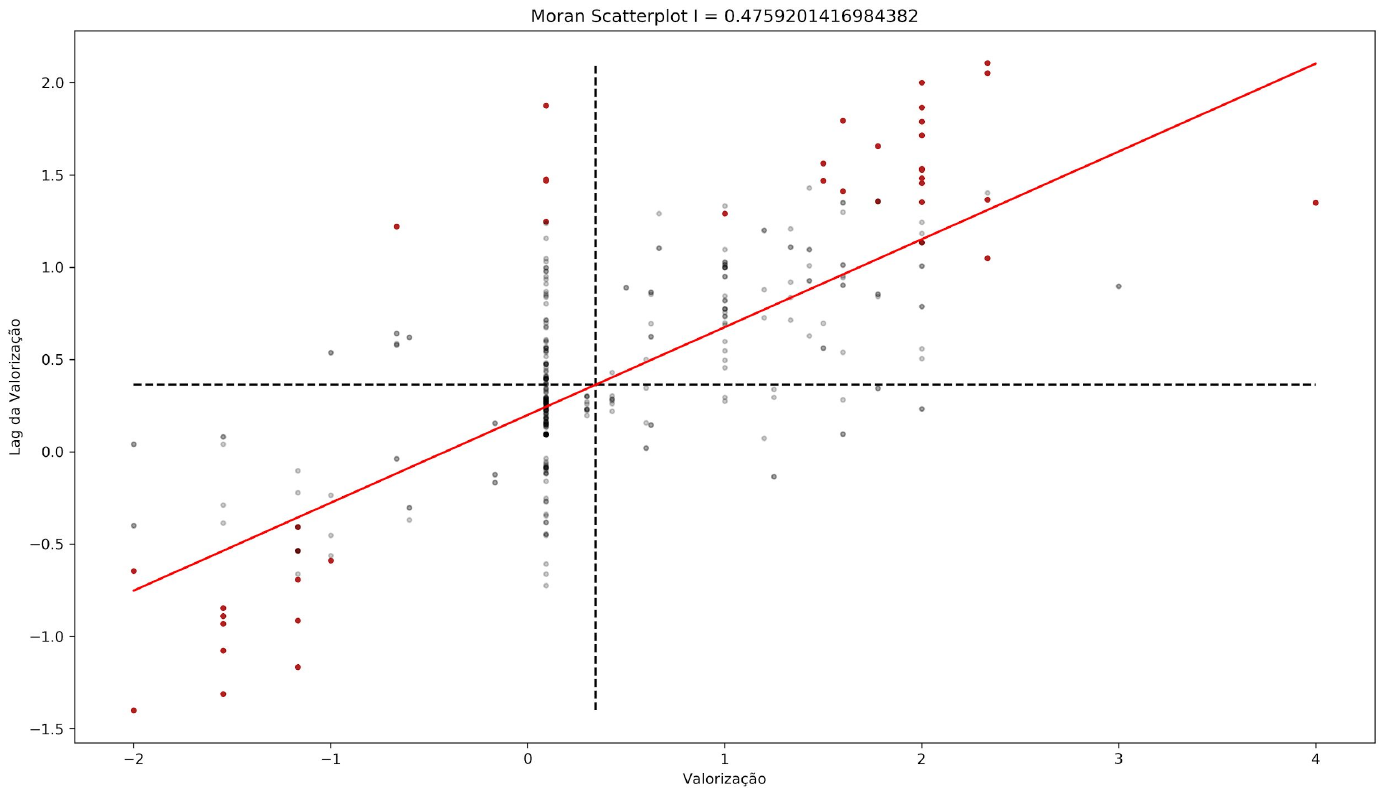
\includegraphics[width=1.0\textwidth]{MoranI}
\par\end{centering}
\caption{\label{fig:moran_i} I de Moran para a valorização em relação ao lag da mesma.} 
\end{figure}
\vspace*{-44pt}
\end{center}

\begin{table}
\begin{lstlisting}[basicstyle={\scriptsize},tabsize=4]
REGRESSION
----------
Data set            :  sao_paulo_renda
SUMMARY OF OUTPUT: ORDINARY LEAST SQUARES ESTIMATION
Dependent Variable  :       RENDA  Number of Observations:  524
Mean dependent var  :     2368.22  Number of Variables   :    2
S.D. dependent var  :      1852.5  Degrees of Freedom    :  522 

R-squared           :    0.027862  F-statistic           :     14.9608
Adjusted R-squared  :    0.026000  Prob(F-statistic)     :  0.00012364
Sum squared residual:1.74813e+009  Log likelihood        :    -4678.85
Sigma-square        :3.34891e+006  Akaike info criterion :      9361.7
S.E. of regression  :        1830  Schwarz criterion     :     9370.22
Sigma-square ML     :3.33613e+006
S.E of regression ML:     1826.51

-----------------------------------------------------------------------------
       Variable      Coefficient      Std.Error    t-Statistic   Probability
-----------------------------------------------------------------------------
          CONSTANT       2326.63        80.6639        28.8436     0.00000
        valorizaca         14432        3731.21        3.86792     0.00012
-----------------------------------------------------------------------------

REGRESSION DIAGNOSTICS  
MULTICOLLINEARITY CONDITION NUMBER   1.143500
TEST ON NORMALITY OF ERRORS
TEST                  DF           VALUE             PROB
Jarque-Bera            2           518.2554          0.00000

RANDOM COEFFICIENTS
DIAGNOSTICS FOR HETEROSKEDASTICITY  
TEST                  DF           VALUE             PROB
Breusch-Pagan test     1             3.9064          0.04810
Koenker-Bassett test   1             1.4837          0.22319
============================== END OF REPORT ================================
\end{lstlisting}

\caption{\label{tab:regression_result} Resultado da regressão de renda em relação a variável valorização.}
\end{table}

\begin{center}
\begin{figure}
\begin{centering}
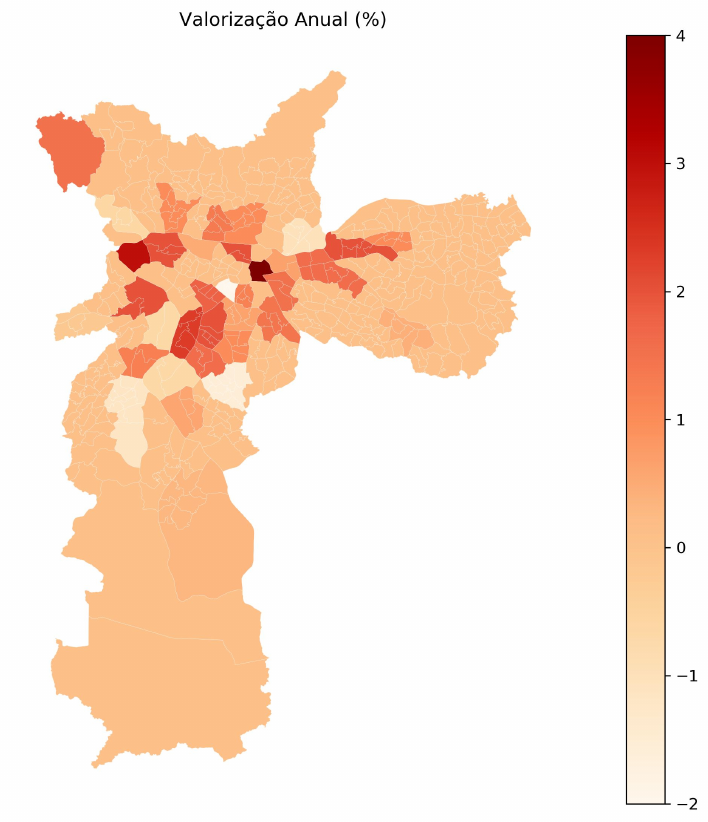
\includegraphics[width=.49\textwidth]{SaoPauloEValuationRegions}
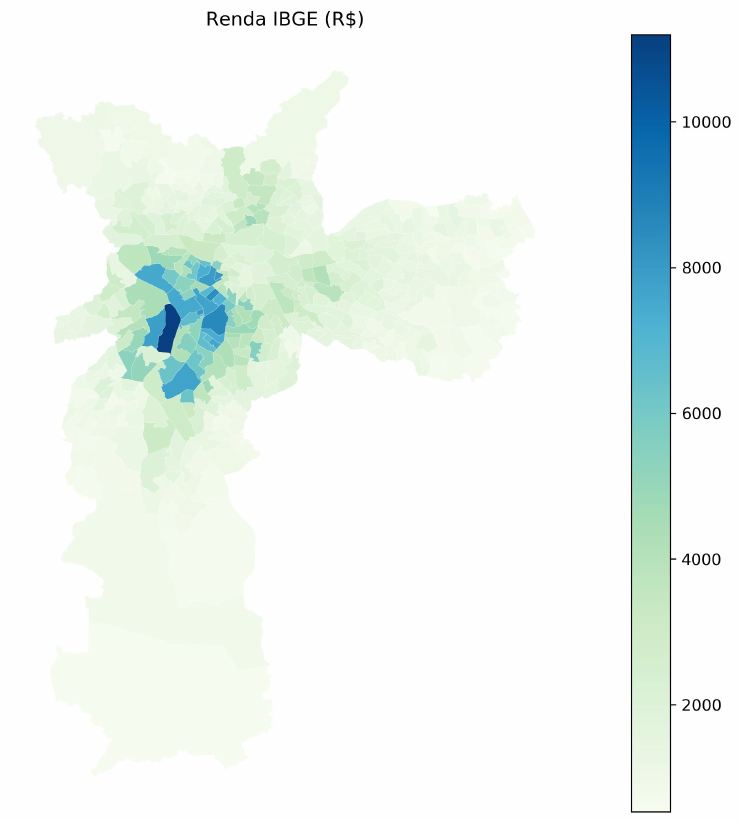
\includegraphics[width=.49\textwidth]{SaoPauloAvgIncome}
\end{centering}
\caption{\label{fig:sao_paulo_stats} À esquerda, o gráfico de valorização na cidade de São Paulo e à direita, o gráfico de salário médio para as regiões censitárias da capital do estado de São Paulo.}
\end{figure}
\end{center}

\begin{center}
\begin{figure}
\begin{centering}
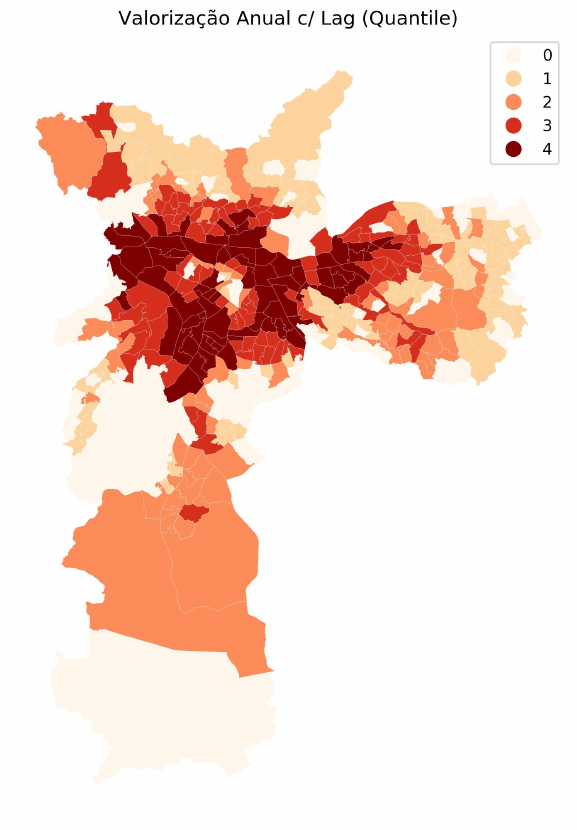
\includegraphics[width=0.6\textwidth]{SaoPauloEvaluationRegionsWithLag}
\par\end{centering}
\caption{\label{fig:sao_paulo_evaluation_with_lag} Valorização anual com lag e vizinhança $n=1$ (Queen). Na legenda apresenta-se a escala em quartis.} 
\end{figure}
\vspace*{-44pt}
\end{center}

A figura~\ref{fig:sao_paulo_stats} mostra tanto o gráfico de valorização anual dos imóveis como os dados censitários do IBGE para as regiões da capital paulistana. Diversas das regiões com renda mais acentuada são também regiões onde a valorização anual dos imóveis se destacou. Sendo assim, é possível entender-se que há uma certa relação intrínseca entre as duas variáveis.

Na figura~\ref{fig:sao_paulo_evaluation_with_lag}, nota-se uma certa difusão ou espalhamento dos efeitos observados na figura~\ref{fig:sao_paulo_stats}. Sendo assim, há para a cidade de São Paulo uma certa razão para os fatores observados.

\subsection{Relação entre Renda e Valorização}
\label{sec:income_evaluation}
Sendo assim observada a relação, será possível traçar-se a relação entre as duas variáveis observadas?

Na tabela~\ref{tab:regression_result}, demonstra-se o resultado da regressão de renda para variável. Nota-se que o $R^{2}$ observado é muito pequeno indicando pouquíssima ou nenhuma correlação. Isto deve-se ao fato, observado na seção~\ref{sec:multivariate_analysis}, que os fundos possuem ativos em diversos distritos e inclusives em diversos estados. 

No caso desta seção, os mesmos fundos possuem ativos em diversos setores de São Paulo, o que implica que o índice final apresentado não é por imóvel, mas sim por fundo. 

Distritos com somente um fundo vão apresentar a valorização do mesmo. Ou seja, é provável que esteja-se alterando o valor esperado do imóvel na região ao analisar-se a performance do fundo em si. 

Para que fosse possível fazer uma análise completa da performance por imóvel, seria interessante acessar o valor base, por imóvel, que compõe o índice final de valorização de cada fundo. Infelizmente, esta informação não está prontamente disponível para utilização nas fontes utilizadas para a extração.

Por fim, a figura~\ref{fig:moran_i}, mostra o I de Moran para a valorização em relação ao seu lag das figuras~\ref{fig:sao_paulo_evaluation_with_lag} e~\ref{fig:sao_paulo_stats}. Este I, apesar de indicar que há correlação espacial também mostra a tendência mencionada anteriormente, na qual diversos distritos, em localizações distintas possuem índices parecidos em função da granularidade dos dados serem por fundo e não por ativo.


\chapter{Conclusion}
\label{chap:conclusion}

Entende-se pelas análises que outras variáveis como segmento e meso-região tem mais influência em um dividendo que a vizinhança em si.

Ainda assim, na cidade de São Paulo, há forte correlação pela análise de vizinhança, indicando que FIIs que tenham ativos na grande São Paulo tem correlação com seus yields e valorização.

O segmento de um FII é um bom fator para mensuração dos possíveis retornos de valorização e yields, conforme graficamente exposto anteriormente.

Assim, a conclusão final do grupo é que para os FIIs, o segmento em que se encontra é um fator descritivo mais forte que a localização dos imóveis. Porém, é possível dizer o mesmo do distrito?

Para fazer-se esta análise, na seção~\ref{sec:spatial_analysis_sao_paulo} obteve-se diversas análises da cidade de São Paulo. Nesta análise, observou-se que a correlação espacial, inexistente no mapa do país como um todo, da seção~\ref{sec:spatial_analysis_br}. 

Demonstrou-se também que diversas das regiões de maior valorização parecem casar com os valores de renda distrital do IBGE. Esta segunda inferência entretanto foi desmentida pela tabela~\ref{tab:regression_result}, onde os resultados da regressão entre renda e valorização demonstram não há correlação qualquer entre as duas variáveis. Sendo assim, não há a possibilidade de usar uma como \emph{proxy} da outra.

Entende-se com isto que a única maneira de poder-se evoluir na análise geoespacial e na inferência de papéis imobiliários a partir de sua localização seria possuir o dado de valorização em sua menor granularidade possível que é o imóvel. Infelizmente, por razões técnicas, a fonte de dados utilizada e obtida por \emph{webscrapping} só admite o índice de valorização por distrito, invalidando as contribuições individuais dos ativos no processo por meio de extração da média global da carteira em questão. 



% ----------------------------------------------------------
% Finaliza a parte no bookmark do PDF
% para que se inicie o bookmark na raiz
% e adiciona espaço de parte no Sumário
% ----------------------------------------------------------
\phantompart

% ----------------------------------------------------------
% ELEMENTOS PÓS-TEXTUAIS
% ----------------------------------------------------------
\postextual
% ----------------------------------------------------------

% ----------------------------------------------------------
% Referências bibliográficas
% ----------------------------------------------------------
\bibliography{referencias}

% ----------------------------------------------------------
% Glossário
% ----------------------------------------------------------
%
% Consulte o manual da classe abntex2 para orientações sobre o glossário.
%
%\glossary

% ----------------------------------------------------------
% Apêndices
% ----------------------------------------------------------

% ---
% Inicia os apêndices
% ---
%\begin{apendicesenv}

%% Imprime uma página indicando o início dos apêndices
%\partapendices

%% ----------------------------------------------------------
%\chapter{Quisque libero justo}
%% ----------------------------------------------------------

%\lipsum[50]

%% ----------------------------------------------------------
%\chapter{Nullam elementum urna vel imperdiet sodales elit ipsum pharetra ligula
%ac pretium ante justo a nulla curabitur tristique arcu eu metus}
%% ----------------------------------------------------------
%\lipsum[55-57]

%\end{apendicesenv}
% ---


% ----------------------------------------------------------
% Anexos
% ----------------------------------------------------------

% ---
% Inicia os anexos
% ---
%\begin{anexosenv}

%% Imprime uma página indicando o início dos anexos
%\partanexos

%% ---
%\chapter{Morbi ultrices rutrum lorem.}
%% ---
%\lipsum[30]

%% ---
%\chapter{Cras non urna sed feugiat cum sociis natoque penatibus et magnis dis
%parturient montes nascetur ridiculus mus}
%% ---

%\lipsum[31]

%% ---
%\chapter{Fusce facilisis lacinia dui}
%% ---

%\lipsum[32]

%\end{anexosenv}

%---------------------------------------------------------------------
% INDICE REMISSIVO
%---------------------------------------------------------------------
\phantompart
\printindex
%---------------------------------------------------------------------

\end{document}
